% =====================================================================
%  Master's internship report — Master in Data Science (Univ. Rouen)
%  Author: Ayoub EL HARRAN — Data Engineering @ Qonto
%  Engine: XeLaTeX (OpenType fonts + polyglossia EN/FR)
%  Build:  latexmk -xelatex main.tex   (or xelatex main.tex ×2)
% =====================================================================
\documentclass[11pt,a4paper,oneside]{report}

% ---------- Language & fonts (XeLaTeX + polyglossia) ----------
\usepackage{polyglossia}
\setmainlanguage{english}
\setotherlanguage{french}
\usepackage{fontspec}
\defaultfontfeatures{Ligatures=TeX}
\setmainfont{TeX Gyre Pagella}
\setsansfont{TeX Gyre Heros}
\setmonofont{Latin Modern Mono}[Scale=0.92]

% ---------- Page layout ----------
\usepackage[a4paper,top=2.6cm,bottom=2.4cm,left=2.6cm,right=2.6cm,headheight=14pt]{geometry}
\usepackage{microtype}
\usepackage{setspace}
\onehalfspacing
\usepackage{emptypage}
\tolerance=2000
\emergencystretch=1.2em

% ---------- Colours ----------
\usepackage{xcolor}
\definecolor{qink}{HTML}{1F2933}
\definecolor{qaccent}{HTML}{1F6FB2}
\definecolor{qaccent2}{HTML}{2B8A6F}
\definecolor{qgray}{HTML}{5B6570}
\definecolor{qlight}{HTML}{EEF3F7}
\definecolor{qcode}{HTML}{F5F7FA}
\definecolor{codekw}{HTML}{0B5FA5}
\definecolor{codestr}{HTML}{2B8A6F}
\definecolor{codecmt}{HTML}{8A94A0}

% ---------- Headings ----------
\usepackage{titlesec}
\titleformat{\chapter}[display]
  {\normalfont\sffamily\bfseries\color{qink}}
  {\raggedright\large\color{qaccent}\MakeUppercase{\chaptertitlename}\ \thechapter}
  {8pt}{\Huge\raggedright}
  [\vspace{4pt}{\color{qaccent}\titlerule[1.2pt]}]
\titlespacing*{\chapter}{0pt}{6pt}{22pt}
\titleformat{\section}
  {\normalfont\sffamily\large\bfseries\color{qink}}{\color{qaccent}\thesection}{0.7em}{}
\titleformat{\subsection}
  {\normalfont\sffamily\normalsize\bfseries\color{qink!90}}{\color{qaccent}\thesubsection}{0.6em}{}

% ---------- Headers / footers ----------
\usepackage{fancyhdr}
\pagestyle{fancy}
\fancyhf{}
\renewcommand{\headrulewidth}{0.4pt}
\fancyhead[L]{\footnotesize\sffamily\color{qgray}\nouppercase{\leftmark}}
\fancyhead[R]{\footnotesize\sffamily\color{qgray}Internship report — Qonto}
\fancyfoot[C]{\footnotesize\sffamily\color{qgray}\thepage}
\renewcommand{\chaptermark}[1]{\markboth{\thechapter.\ #1}{}}

% ---------- Lists, tables, figures ----------
\usepackage{enumitem}
\setlist{itemsep=2pt,topsep=3pt,parsep=0pt}
\usepackage{booktabs}
\usepackage{tabularx}
\usepackage{array}
\usepackage{graphicx}
\usepackage{float}
\usepackage{caption}
\captionsetup{font=small,labelfont={sf,bf,color=qaccent},textfont=sf}

% ---------- Callout boxes ----------
\usepackage[most]{tcolorbox}
\newtcolorbox{keybox}[1][Results]{
  colback=qlight,colframe=qaccent,coltitle=white,
  fonttitle=\sffamily\bfseries,title={#1},
  boxrule=0.8pt,arc=2pt,left=6pt,right=6pt,top=4pt,bottom=4pt,breakable}
\newtcolorbox{contribbox}[1][My contribution]{
  colback=qaccent2!8,colframe=qaccent2,coltitle=white,
  fonttitle=\sffamily\bfseries,title={#1},
  boxrule=0.8pt,arc=2pt,left=6pt,right=6pt,top=4pt,bottom=4pt,breakable}

% ---------- Code ----------
\usepackage{listings}
\lstset{
  basicstyle=\ttfamily\footnotesize,
  backgroundcolor=\color{qcode},
  keywordstyle=\color{codekw}\bfseries,
  stringstyle=\color{codestr},
  commentstyle=\color{codecmt}\itshape,
  numberstyle=\tiny\color{qgray},
  numbers=left,numbersep=7pt,
  frame=single,rulecolor=\color{qgray!35},
  breaklines=true,breakatwhitespace=false,
  showstringspaces=false,tabsize=2,
  captionpos=b,columns=fullflexible,
  aboveskip=8pt,belowskip=6pt,
  literate={é}{{\'e}}1 {è}{{\`e}}1 {à}{{\`a}}1 {ê}{{\^e}}1 {ç}{{\c c}}1 {’}{{'}}1 {→}{{$\rightarrow$}}1 {–}{{-}}1
}
\lstdefinelanguage{yaml}{
  keywords={true,false,null,dags,tasks,type,options,depends_on,schedule,owner,env_vars},
  keywordstyle=\color{codekw}\bfseries,
  comment=[l]{\#},morecomment=[l]{\#},
  morestring=[b]",morestring=[b]'
}

% ---------- Misc ----------
\usepackage{csquotes}
\usepackage{tikz}
\usetikzlibrary{shapes.geometric,arrows.meta,positioning,fit,backgrounds,calc}
\usepackage{pgfplots}\pgfplotsset{compat=1.17}
\usepackage[hidelinks,colorlinks=true,linkcolor=qink,urlcolor=qaccent,citecolor=qaccent]{hyperref}
\usepackage{bookmark}

% =====================================================================
%  COVER VARIABLES — TO BE COMPLETED BY AYOUB (placeholders)
% =====================================================================
\newcommand{\studentName}{Ayoub ELHARRAN}
\newcommand{\studentTrack}{Master 2 — Data Science and Engineering}
\newcommand{\academicYear}{Academic year 2025--2026}
\newcommand{\reportTitle}{Decouple to harden:\\ migrating and industrialising data pipelines at Qonto}
% \newcommand{\reportSubtitle}{Notion ingestion \textrightarrow{} dlt, Tableau DAGs \& JWT authentication, and CESOP Netherlands regulatory transmission}
\newcommand{\reportSubtitle}{}
\newcommand{\companyName}{Qonto (Olinda SAS)}
\newcommand{\companyTutor}{Michael Ourch}
\newcommand{\companyTutorRole}{Senior Data Engineer, Data Platform}
\newcommand{\companyTutorMail}{michael.ourch@qonto.com}
\newcommand{\companyAddress}{\textcolor{qgray}{}}
\newcommand{\universityTutor}{Maxime Berar}
\newcommand{\internshipPeriod}{April -- October 2026}
\newcommand{\university}{Université de Rouen Normandie \textemdash{} UFR of Sciences and Technology}

% =====================================================================
\begin{document}
\pagenumbering{roman}
% ---------------- Cover page ----------------
\begin{titlepage}
\thispagestyle{empty}
\centering
\vspace*{0.4cm}

{\sffamily\large\color{qgray} \university\par}
{\sffamily\normalsize\color{qgray} \academicYear\par}

\vspace{0.5cm}
{\color{qaccent}\rule{\textwidth}{1.4pt}}
\vspace{1.4cm}

{\sffamily\bfseries\color{qink}\fontsize{15}{18}\selectfont Master's end-of-studies internship report\par}
\vspace{0.3cm}
{\sffamily\color{qgray}\large \studentTrack\par}

\vspace{1.6cm}
{\sffamily\bfseries\color{qink}\fontsize{23}{27}\selectfont \reportTitle\par}
\vspace{0.7cm}
{\sffamily\itshape\color{qaccent}\large \reportSubtitle\par}

\vspace{1.6cm}
{\color{qaccent}\rule{0.5\textwidth}{0.8pt}}
\vspace{1.2cm}

\begin{tabular}{@{}r@{\hskip 10pt}l@{}}
\sffamily\bfseries\color{qink} Student & \sffamily \studentName \\[4pt]
\sffamily\bfseries\color{qink} Company & \sffamily \companyName \\[4pt]
\sffamily\bfseries\color{qink} Period & \sffamily \internshipPeriod \\[4pt]
\sffamily\bfseries\color{qink} Company supervisor & \sffamily \companyTutor \\
 & \sffamily\small\color{qgray} \companyTutorRole \\
 & \sffamily\small\color{qgray} \companyTutorMail \\
 & \sffamily\small\color{qgray} \companyAddress \\[4pt]
\sffamily\bfseries\color{qink} University tutor & \sffamily \universityTutor \\
\end{tabular}

\vfill
{\color{qaccent}\rule{\textwidth}{1.4pt}}
\vspace{0.3cm}
{\sffamily\footnotesize\color{qgray} Data Platform team — Data Engineering \quad$\bullet$\quad \companyName\par}
\end{titlepage}

% ---------------- Abstract / Résumé ----------------
\chapter*{Abstract}
\addcontentsline{toc}{chapter}{Abstract}
\markboth{Abstract}{}

This end-of-studies internship took place within Qonto's \emph{Data Platform} team, a European neobank and payment service provider (PSP). It focused on hardening and industrialising data pipelines orchestrated by Apache Airflow. Three projects are presented. The first is the migration of Notion data ingestion to the \emph{dlt} (data load tool) framework with a direct Snowflake destination: it was triggered by a \emph{silent data-truncation} incident caused by an API change, and its core challenge was achieving \emph{byte-for-byte} parity with the legacy system so that the production cutover would be downtime-free and transparent to the hundreds of downstream dbt models. The second project replaced personal-access-token authentication (14 manually rotated PATs relying on a brittle pooling mechanism) with a JWT-based \emph{Connected App} (a single secret), while moving the Tableau pipelines out of Airflow's shared Docker base image. The third, being finalised, implements the \emph{CESOP Netherlands} regulatory transmission chain to the government Digipoort gateway over FTPS/mTLS with a PKIoverheid certificate, as two DAGs (a quarterly submitter and an asynchronous receipt poller). The common thread of the first two projects is \emph{decoupling} a shared infrastructure dependency, identified as the true source of fragility, before fixing the business problem itself. Results include eliminating silent truncation by construction, removing all manual token rotation, and substantially reducing legacy code and the number of Airflow tasks.

\vspace{4pt}
\noindent\textbf{Keywords:} data engineering, Apache Airflow, dlt, Snowflake, dbt, EL ingestion, orchestration, JWT authentication, mTLS/PKI, regulatory compliance (CESOP), zero-downtime migration.

\clearpage
\begin{french}
\chapter*{Résumé}
\addcontentsline{toc}{chapter}{Résumé}
\markboth{Résumé}{}

Ce stage de fin d'études s'est déroulé au sein de l'équipe \emph{Data Platform} de Qonto, néobanque européenne et prestataire de services de paiement (PSP). Il portait sur la fiabilisation et l'industrialisation de pipelines de données orchestrés par Apache Airflow. Trois projets y sont présentés. Le premier est la migration de l'ingestion des données Notion vers le framework \emph{dlt} (data load tool) avec écriture directe dans Snowflake : le déclencheur était un incident de \emph{troncature silencieuse} causé par un changement d'API, et la difficulté centrale a été d'obtenir une parité \emph{octet-à-octet} avec l'ancien système pour réaliser une bascule de production sans interruption ni régression sur les modèles dbt en aval. Le deuxième projet a remplacé l'authentification par jetons personnels (14 PAT à rotation manuelle, avec un mécanisme de pool fragile) par une \emph{Connected App} en JWT (un unique secret), tout en migrant les pipelines Tableau hors de l'image Docker partagée d'Airflow. Le troisième, en cours de finalisation, met en place la chaîne de transmission réglementaire \emph{CESOP Pays-Bas} vers la passerelle gouvernementale Digipoort en FTPS/mTLS avec certificat PKIoverheid, sous la forme de deux DAGs. Le fil conducteur des deux premiers projets est le \emph{découplage} d'une dépendance d'infrastructure partagée, identifiée comme la véritable cause de fragilité, avant la correction du problème métier.

\vspace{4pt}
\noindent\textbf{Mots-clés :} ingénierie des données, Apache Airflow, dlt, Snowflake, dbt, ingestion EL, orchestration, authentification JWT, mTLS/PKI, conformité réglementaire (CESOP), migration sans interruption.
\end{french}

% ---------------- Acknowledgements ----------------
\chapter*{Acknowledgements}
\addcontentsline{toc}{chapter}{Acknowledgements}
\markboth{Acknowledgements}{}

I would like to thank the entire \emph{Data Platform} team at Qonto for their welcome and the trust they placed in me throughout this internship.

My thanks go first to my company supervisor, \companyTutor{}, for the mentoring, the quality of the code reviews, and the latitude I was given to take ownership of high-impact, production-facing topics.

I also thank the team's engineers for their availability, their demanding reviews, and the technical discussions that shaped each of the projects presented in this report, as well as the \emph{Regulatory} team with whom I collaborated on the CESOP project.

Finally, I express my gratitude to \universityTutor{}, my university tutor, and to the teaching team of the \university{}, for their guidance and advice during this final year of the master's programme.

\microtypesetup{protrusion=false}
\tableofcontents
\microtypesetup{protrusion=true}
\cleardoublepage
% ---------------- Glossary ----------------
\chapter*{Glossary \& acronyms}
\addcontentsline{toc}{chapter}{Glossary \& acronyms}
\markboth{Glossary}{}

\begin{description}[style=nextline,leftmargin=1em,font=\sffamily\bfseries\color{qink}]
  \item[Airflow] Open-source workflow orchestrator. A pipeline is described as a \textbf{DAG}.
  \item[DAG] \emph{Directed Acyclic Graph}: a scheduled pipeline, a set of tasks linked by dependencies.
  \item[dbt] \emph{data build tool}: SQL transformation tool running downstream of the data warehouse.
  \item[dlt] \emph{data load tool}: a Python \textbf{EL} ingestion library (extract + load) with automatic normalisation, staging and loading.
  \item[EL / ETL] Data-integration paradigms: \emph{Extract–Load} (transformation deferred downstream) vs \emph{Extract–Transform–Load}.
  \item[Snowflake] Cloud data warehouse, the target of every ingestion.
  \item[S3] Amazon Web Services object storage, used as a \emph{staging} area.
  \item[Data contract (Qontract)] A YAML file declaring the fields, types and key of an ingested table.
  \item[Job Orchestrator] Qonto-internal pattern: a job is declared in a \texttt{schedule.yaml} and its Airflow DAG is \emph{auto-generated}, in a repository and Docker image dedicated to that job.
  \item[PAT] \emph{Personal Access Token}: a personal token with limited lifetime and manual rotation.
  \item[JWT] \emph{JSON Web Token}: a signed token, used here via a Tableau \emph{Connected App} for authentication.
  \item[Connected App] A trusted application declared on the Tableau side, enabling signed-JWT authentication instead of PATs.
  \item[mTLS] \emph{mutual TLS}: authentication in which both client and server present a certificate.
  \item[PKIoverheid] The Dutch government's public-key infrastructure; issues trusted X.509 certificates.
  \item[Digipoort] The Dutch government's file-exchange gateway (operated by Logius).
  \item[FTPS] \emph{FTP over TLS} (RFC 4217) — not to be confused with SFTP (FTP over SSH).
  \item[CESOP] \emph{Central Electronic System of Payment information}: the EU system for collecting cross-border payment data (VAT anti-fraud).
  \item[PSP] \emph{Payment Service Provider} (Qonto's status).
  \item[PR] \emph{Pull Request}: a proposed code change submitted for review.
  \item[VARIANT] Snowflake's semi-structured type (stores native JSON / arrays / objects).
\end{description}


\cleardoublepage
\pagenumbering{arabic}
% ================= Introduction =================
\chapter*{Introduction}
\addcontentsline{toc}{chapter}{Introduction}
\markboth{Introduction}{}

Data sits at the heart of how a financial company operates: it feeds steering, fraud detection, customer relationship management and, increasingly, regulatory obligations. At Qonto, a European neobank and payment service provider, hundreds of data flows converge every night into a Snowflake warehouse, where they are transformed and then exposed to business teams. These flows are orchestrated by Apache Airflow. Their reliability directly conditions the quality of downstream decisions: a wrong figure, an incomplete table or an unrefreshed dashboard all have concrete consequences.

My end-of-studies internship took place within the \emph{Data Platform} team, whose mission is precisely to build and maintain this ingestion, transformation and delivery infrastructure. The initial topic was about hardening existing pipelines that were quickly crystallised around a recurring observation: several jobs historically written \emph{inside} the monolithic \texttt{qonto-airflow} repository and its shared Docker image suffered from the same structural weakness. That image, common to every pipeline, made any library upgrade risky (it could affect all flows) and concealed silent failures. The problem statement of this internship can therefore be phrased as follows:

\begin{quote}
\itshape How can we harden and industrialise business-critical data pipelines, without any service interruption for their consumers, when the true source of fragility is not the business logic but a shared infrastructure dependency?
\end{quote}

This report presents three projects carried out in response to that question. The first two share a common pattern: diagnosing that the real constraint is the coupling to the Airflow image, \emph{decoupling} the job into a dedicated repository and image, then taking the opportunity to remove a brittle legacy mechanism. The first project migrates Notion ingestion to the \emph{dlt} framework in response to a silent-truncation incident; the second replaces hard-to-maintain personal-token authentication with a JWT-based \emph{Connected App} for the Tableau pipelines. The third project, of a different nature, consists in building a brand-new regulatory transmission chain (the CESOP filing for the Netherlands) to a government gateway that imposes a specific exchange protocol and authentication scheme.

The report is organised as follows. \textbf{Chapter~\ref{ch:context}} introduces the company, the team and the technical ecosystem in which the projects take place, together with the working method. \textbf{Chapter~\ref{ch:sota}} reviews the state of the art of the relevant ingestion, orchestration and authentication approaches, and formalises the common problem. \textbf{Chapters~\ref{ch:notion}, \ref{ch:tableau} and~\ref{ch:cesop}} detail the three projects, each following the same outline: the legacy, the problem, the options considered and the decision, the implementation, the difficulties encountered and the evaluation of results. \textbf{Chapter~\ref{ch:assessment}} draws up an assessment of the skills acquired. The conclusion revisits the main lessons and outlines perspectives.

Throughout the report, particular care is taken to distinguish teamwork from my \emph{personal contribution}, as recommended by the assessment guidelines, and to \emph{measure}, wherever possible, the effects of the changes introduced.

\chapter{Internship context}\label{ch:context}

This chapter introduces the host company, the team I worked in, the technical ecosystem underpinning the projects, and the working method. It provides the background needed to understand the following chapters.

\section{The company: Qonto}

Qonto is a European neobank for freelancers, very small businesses and SMEs. Founded in 2017 by Alexandre Prot and Steve Anavi, it is operated by the company Olinda~SAS and offers a business account together with financial-management services: payment cards, transfers, invoicing, pre-accounting and steering tools~\cite{qonto-wiki,qonto-press}. At the time of the internship, Qonto reports on the order of 600{,}000 customers and operates in eight European countries: France, Germany, Italy, Spain, Austria, Belgium, the Netherlands and Portugal, following an expansion into four new markets in 2024~\cite{qonto-press}.

On the regulatory side, Qonto operates as a \emph{payment institution} (Payment Service Provider, PSP). This status is not a mere legal detail: it entails regulatory-reporting obligations, including the European CESOP filing addressed in Chapter~\ref{ch:cesop} and demands a high level of rigour on data reliability and traceability. The opening of a Dutch IBAN in late 2025 is precisely what made Qonto liable for the CESOP filing in the Netherlands.

\begin{figure}[H]
\centering

\includegraphics[width=0.6\textwidth]{imgs/qonto.png}
\caption{Qonto logo}
\label{fig:qonto-way-card}
\end{figure}

\section{The Data Platform team and the Qonto Way}

I completed my internship within the \emph{Data Platform} team, part of the Data department. Its mission is to provide business and other technical teams with a reliable platform for ingesting, transforming and delivering data. It owns the ``plumbing'': moving data from dozens of sources into the warehouse, guaranteeing its freshness and accuracy, and exposing the results.

Each initiative is run as a Notion \emph{project card} following the \emph{Qonto Way}, a structured lifecycle in three phases (Figure~\ref{fig:qonto-way-card}). \textbf{Value Analysis} (VA) frames the problem: an \emph{Intro \& Context}, the \emph{Definition of Done}, and the \emph{Goals}. \textbf{Value Engineering} (VE) designs the solution: a \emph{Visual Spec}, the \emph{Hard Points} (the open questions or blockers to resolve before building), the \emph{Solutions}, and a \emph{Dive-in} holding the deep implementation notes. \textbf{Build} then executes the work as a task kanban (\emph{Not started} / \emph{In progress} / \emph{Done}). I followed this method for all three projects; the card in Figure~\ref{fig:qonto-way-card} is the real one for the Tableau migration (Chapter~\ref{ch:tableau}).

\begin{figure}[H]
\centering
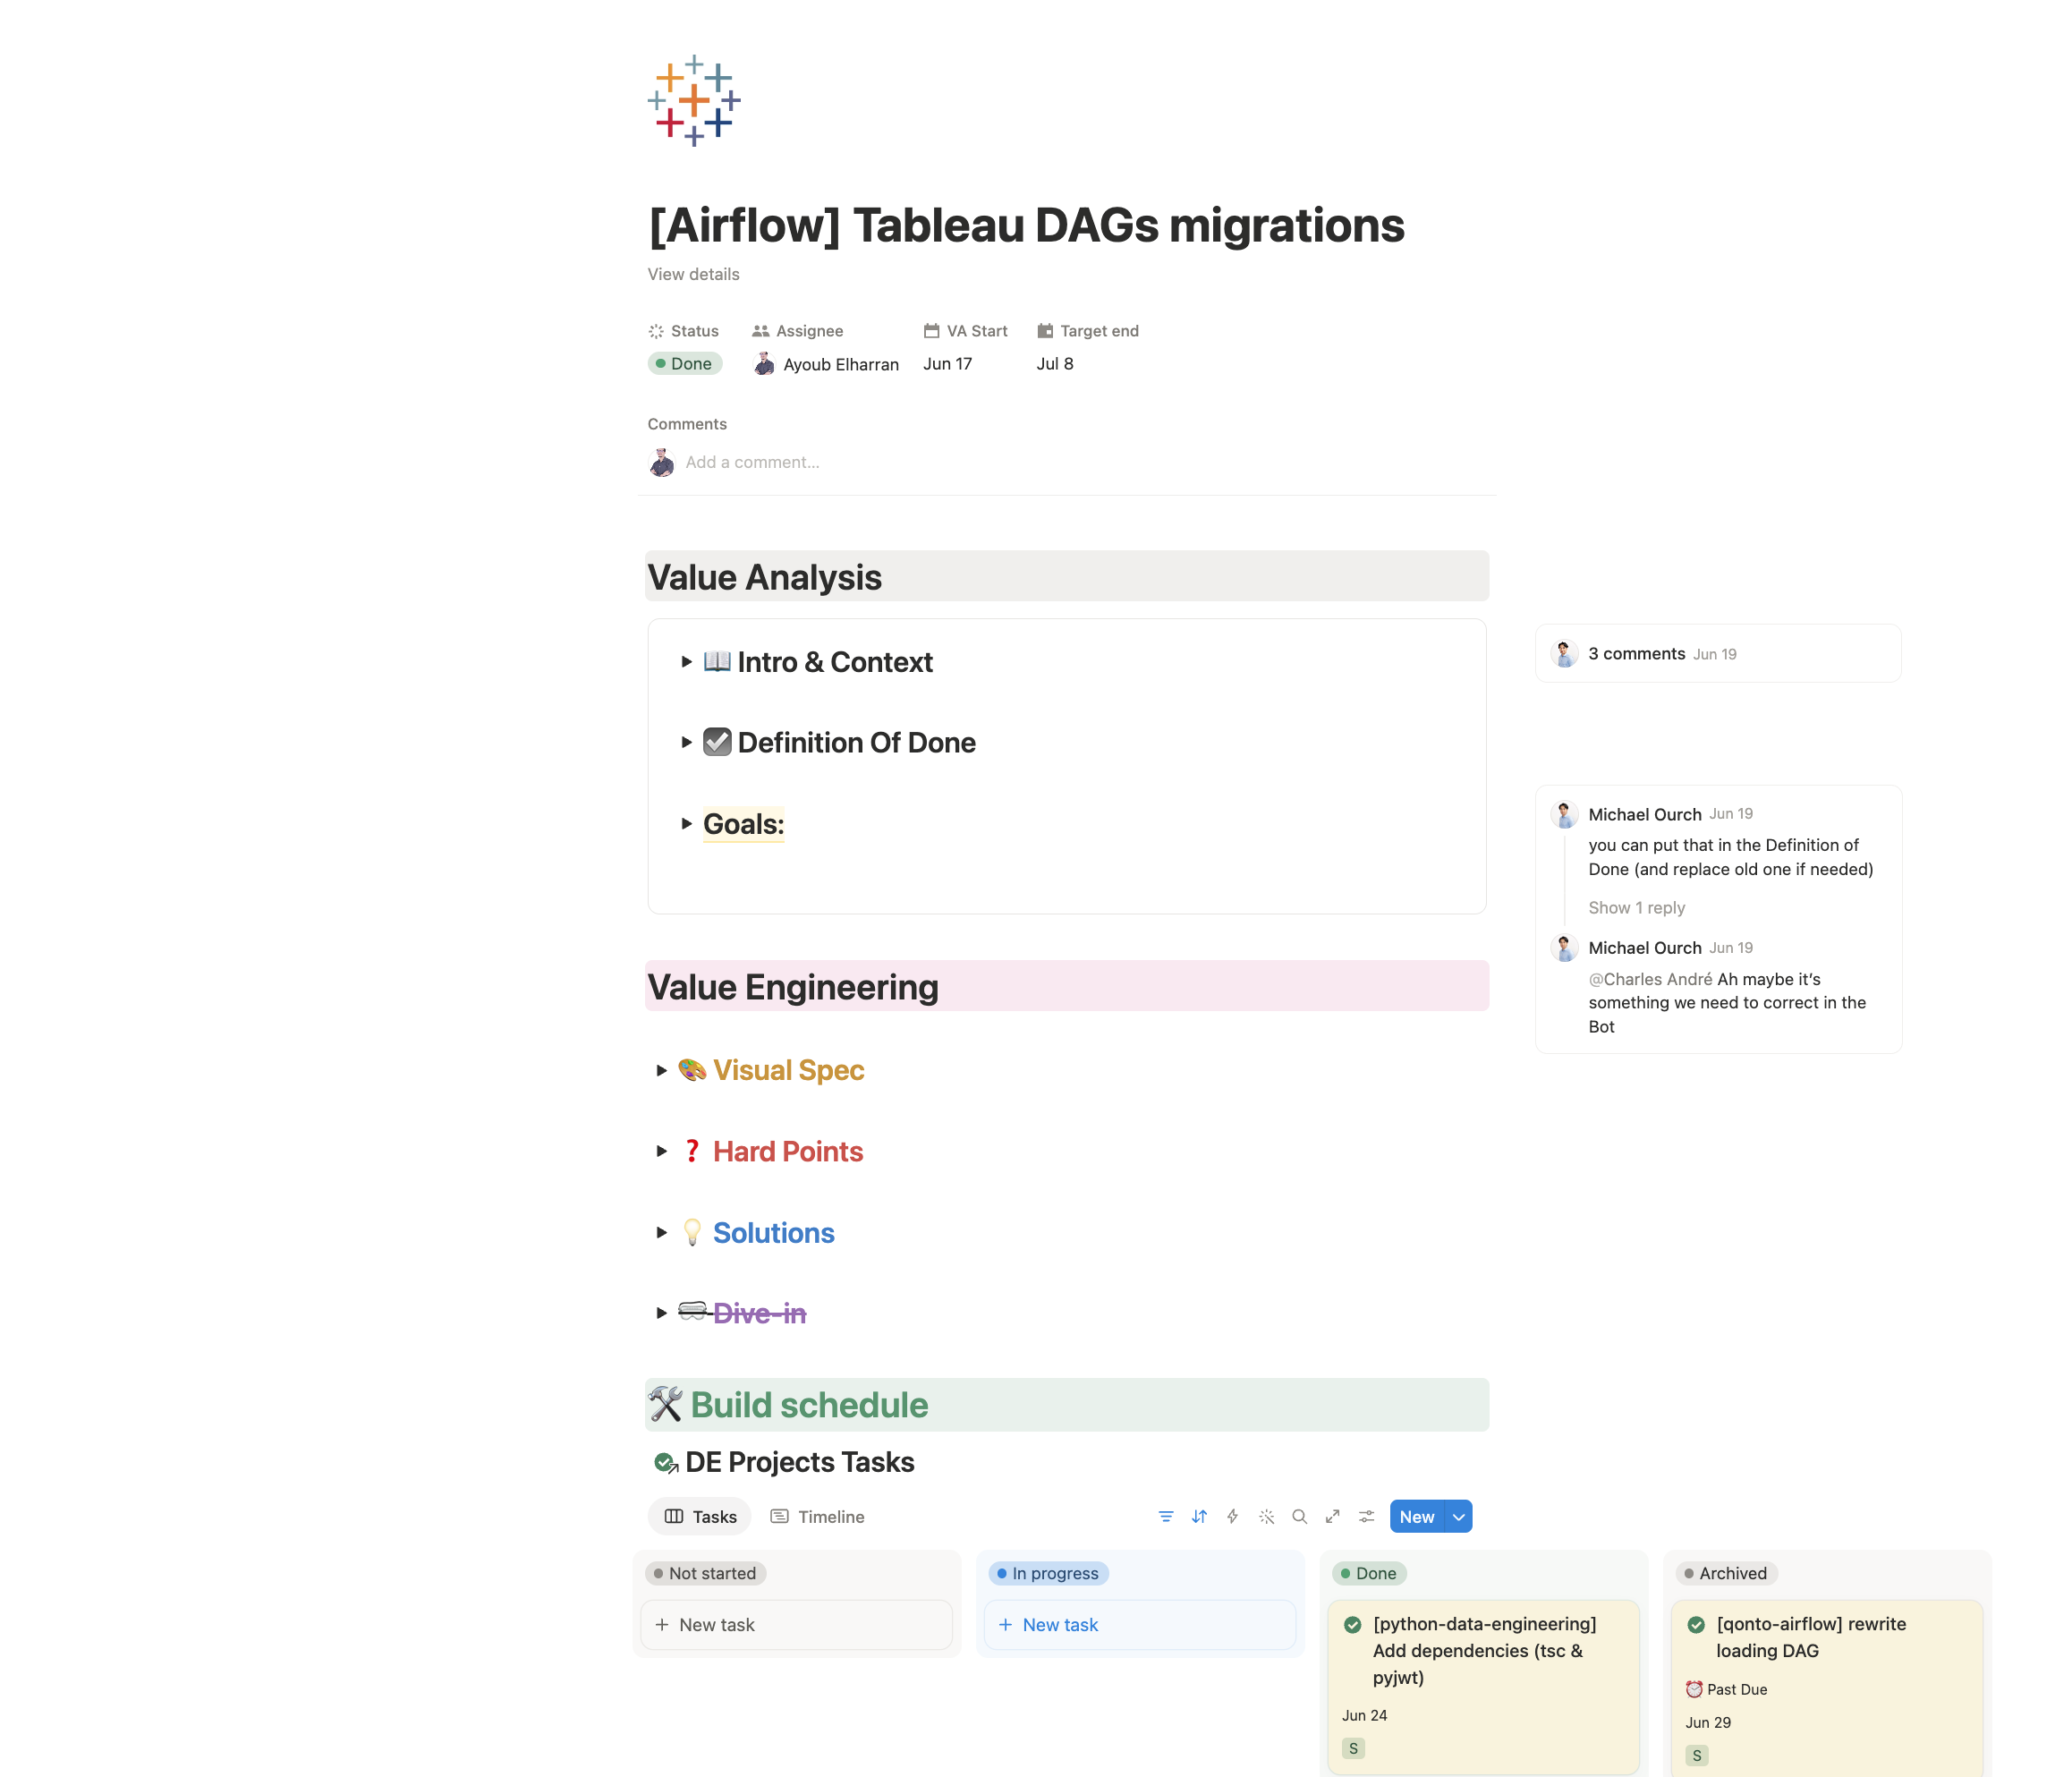
\includegraphics[width=0.8\textwidth]{imgs/project_card_page.png}
\caption{The Notion project card that structures the work following ``the Qonto Way''.}
\label{fig:qonto-way-card}
\end{figure}

At team level, a \emph{Delivery Board} tracks every project across the same lifecycle stages, \emph{Value Analysis} $\rightarrow$ \emph{Value Engineering} $\rightarrow$ \emph{Build} $\rightarrow$ \emph{Value Validation}, each with its blockers and a target date, and reviewed in a daily stand-up (Figure~\ref{fig:delivery-board}). This gave a shared, at-a-glance picture of where each initiative stood. In practice the method strongly structured my work: it forced me to pin down the \emph{Definition of Done} before coding, to surface the \emph{Hard Points} early, and to make trade-offs explicit in the \emph{Solutions} and \emph{Dive-in} sections, a discipline reflected throughout this report.

\begin{figure}[H]
\centering
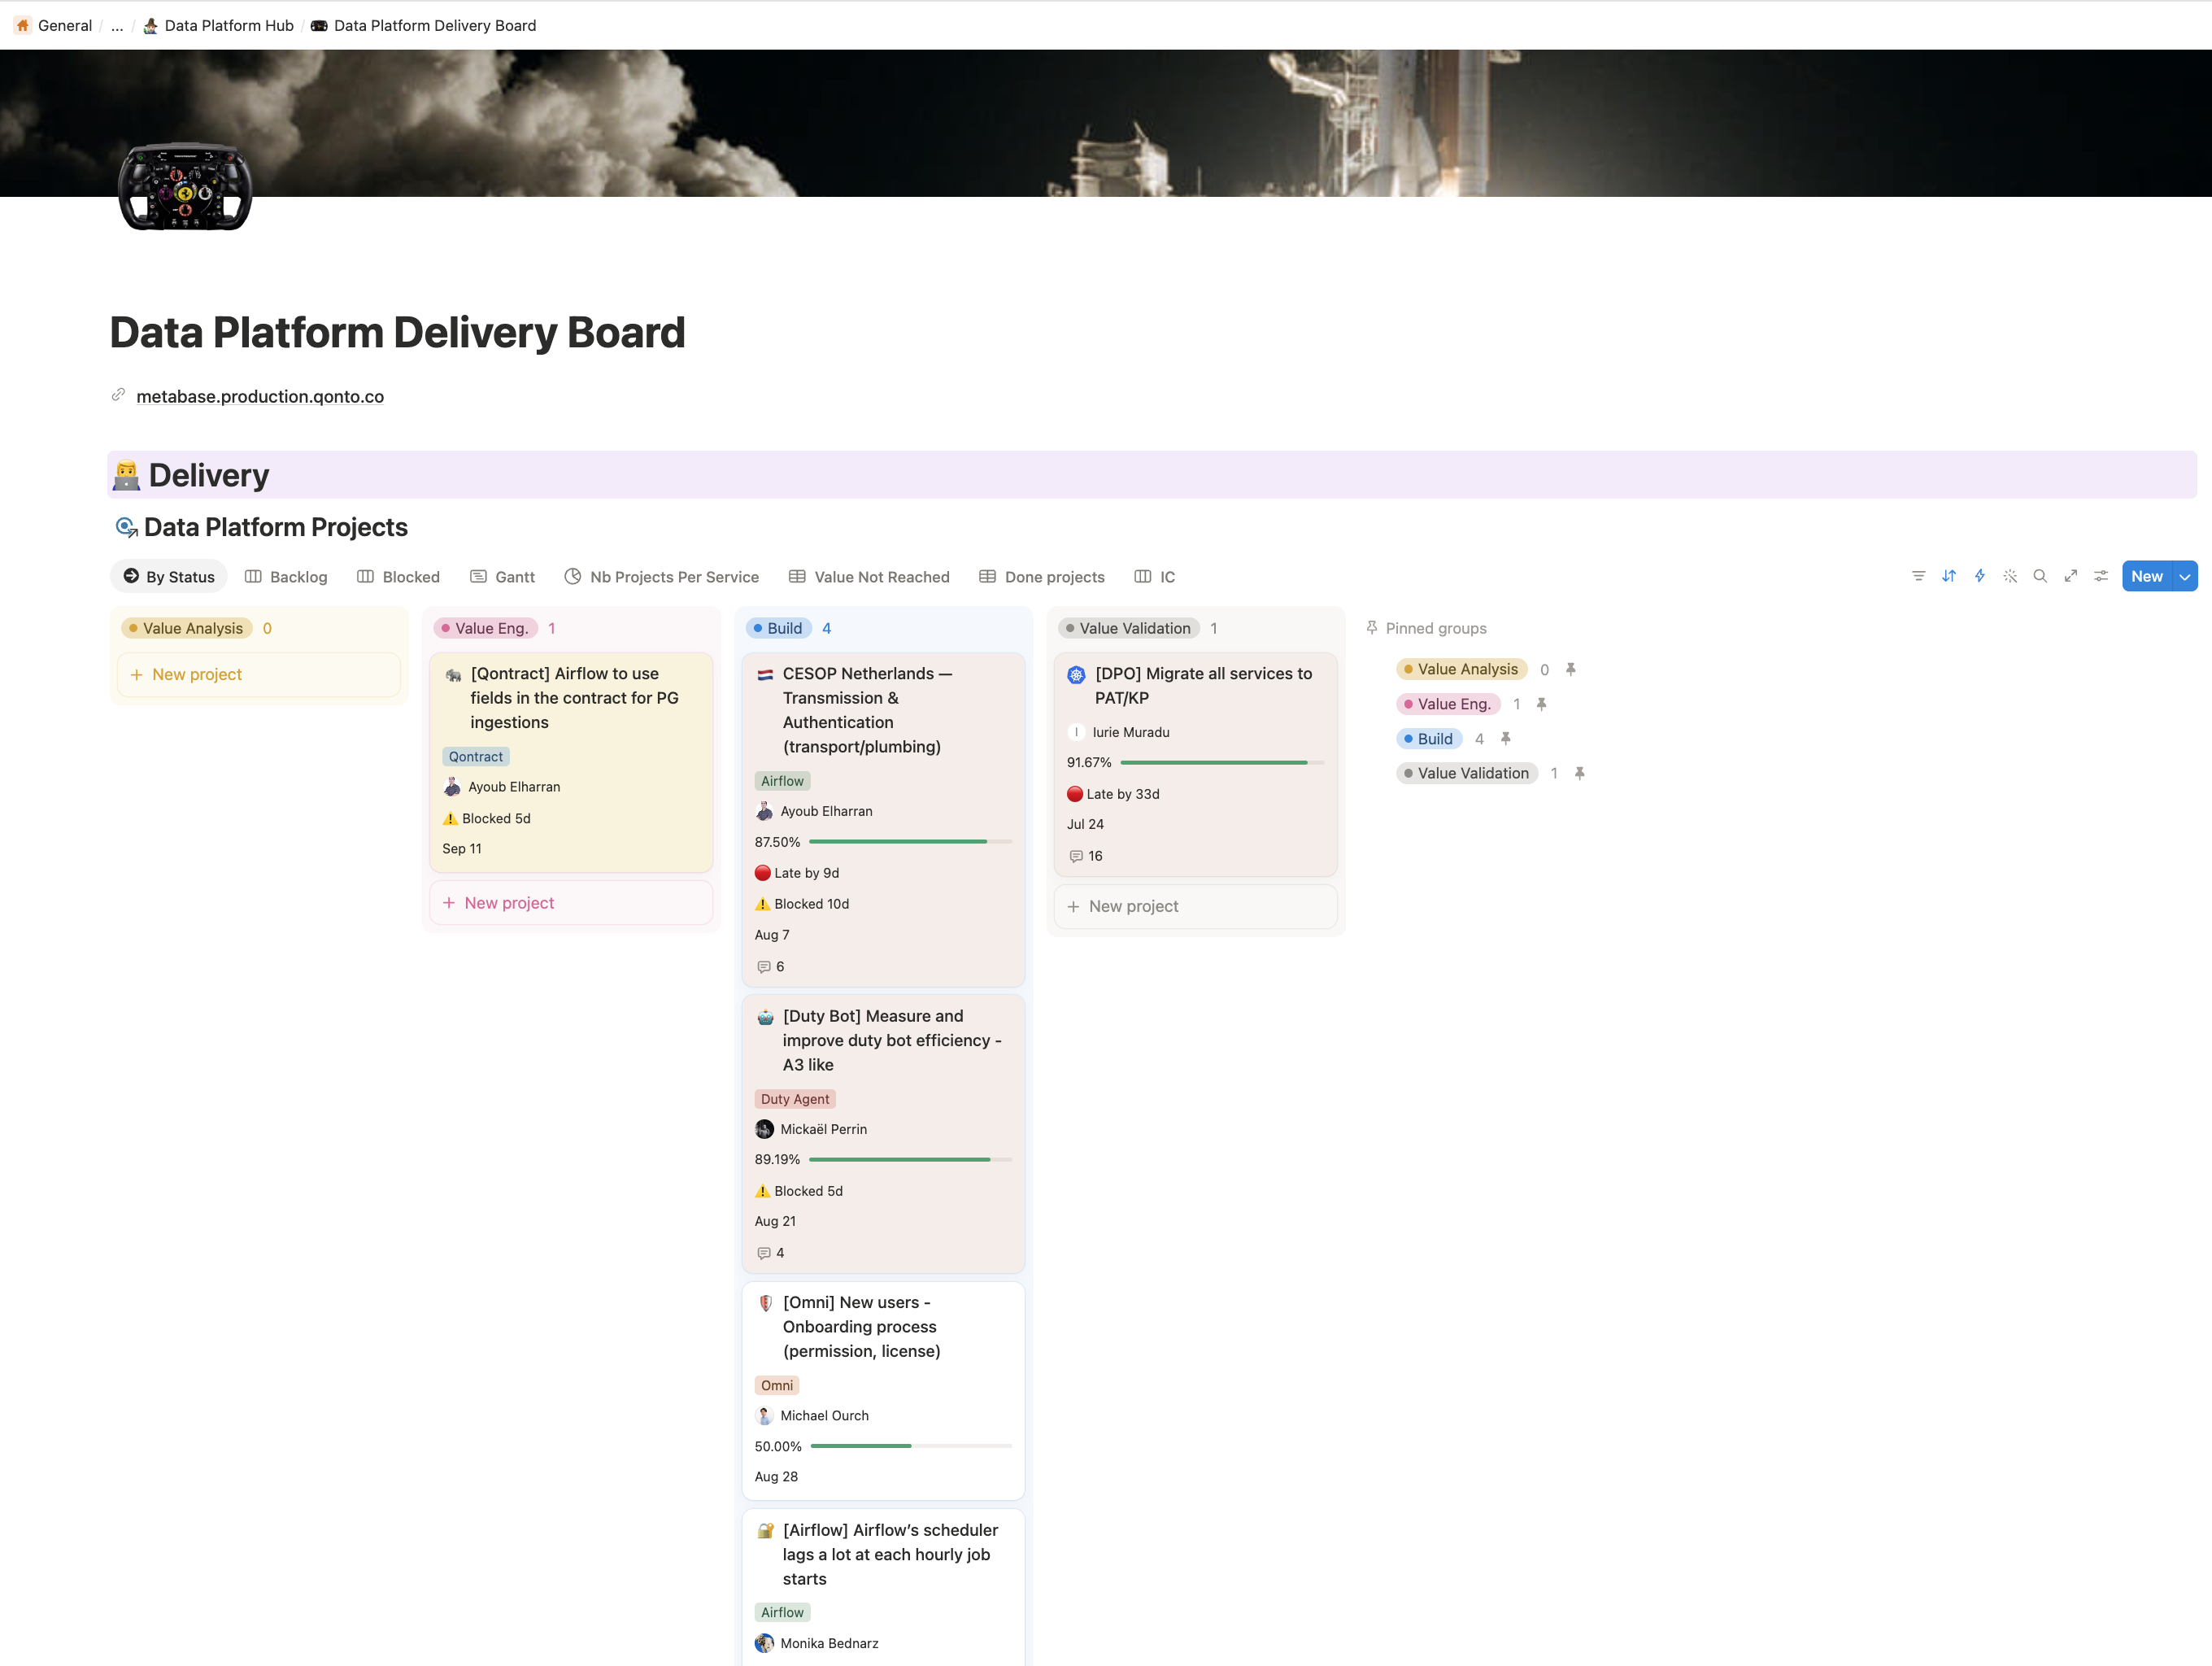
\includegraphics[width=0.8\textwidth]{imgs/data_platform_delivery_board.png}
\caption{The Data Platform Delivery Board}
\label{fig:delivery-board}
\end{figure}

On the engineering side, work goes through \emph{Pull Requests} (PRs) systematically reviewed by one or more engineers, continuous integration (tests, linting, schema validation) and a deployment across successive environments (\emph{staging} then production). This review discipline proved decisive, in particular for the zero-downtime production cutovers described later.


\section{The technical ecosystem}

The ecosystem revolves around a few building blocks (Figure~\ref{fig:archi-platform}):

\begin{itemize}
  \item \textbf{Apache Airflow} is the central orchestrator. Its code lives in a monolithic repository, \texttt{qonto-airflow}, whose distinctive feature is a \emph{declarative} generation model: rather than hand-writing each DAG, one drops a configuration file and the corresponding DAG is produced automatically. This repository relies on a \textbf{shared Docker base image} used by all pipelines; a central point for what follows.
  \begin{figure}[H]
  \centering
  
\includegraphics[width=0.2\textwidth]{imgs/airflow.png}
  \caption{Airflow logo}
  \end{figure}

  \item \textbf{Snowflake} is the cloud data warehouse, the final target of every ingestion. Raw data lands in a \texttt{RAW} database, organised by schema (one per source).
  
  \begin{figure}[H]
  \centering
  
\includegraphics[width=0.2\textwidth]{imgs/Snowflake.png}
  \caption{Snowflake logo}
  \end{figure}

  \item \textbf{Amazon S3} serves as a \emph{staging} area: extractions are written there (CSV, JSONL, Parquet) before being loaded into Snowflake with a \texttt{COPY INTO} command.
  
  \begin{figure}[H]
  \centering
  
\includegraphics[width=0.2\textwidth]{imgs/s3.png}
  \caption{Amazon S3 logo}
  \end{figure}

  \item \textbf{DBT} (\emph{data build tool}) handles downstream transformation: from the \texttt{RAW} tables, SQL models build the business tables consumed by analysts. A single DAG, \texttt{daily\_transform\_dbt}, materialises all these models with their dependencies.
  
  \begin{figure}[H]
  \centering
  \includegraphics[width=0.2\textwidth]{imgs/DBT.png}
  \caption{DBT logo}
  \end{figure}
  
  \item \textbf{Data contracts} (\emph{Qontract}) describe, as YAML files, the expected schema of each ingested table: fields, types, primary key. They are the source of truth for typing.
  \begin{figure}[H]
  \centering
  
\includegraphics[width=0.4\textwidth]{imgs/Qontract.png}
  \caption{Qontract logo}
  \end{figure}
\end{itemize}

\begin{figure}[H]
\centering
\begin{tikzpicture}[
  font=\sffamily\footnotesize,
  node distance=8mm and 12mm,
  box/.style={rectangle,rounded corners=2pt,draw=qgray!60,fill=qlight,minimum height=8mm,minimum width=20mm,align=center,inner sep=4pt},
  src/.style={box,fill=white},
  store/.style={box,fill=qaccent!12,draw=qaccent!70},
  proc/.style={box,fill=qaccent2!12,draw=qaccent2!70},
  arr/.style={-{Stealth[length=2mm]},draw=qgray,thick}
]
\node[src] (sources) {Sources\\{\scriptsize Notion, Tableau,}\\{\scriptsize APIs, Postgres\dots}};
\node[proc,right=of sources] (airflow) {Airflow\\{\scriptsize (ingestion)}};
\node[store,right=of airflow] (s3) {S3\\{\scriptsize staging}};
\node[store,right=of s3] (raw) {Snowflake\\\texttt{RAW}};
\node[proc,below=10mm of raw] (dbt) {dbt\\{\scriptsize transform}};
\node[store,left=of dbt] (marts) {Snowflake\\{\scriptsize marts}};
\node[src,left=of marts] (bi) {Delivery\\{\scriptsize Tableau, exports}};
\draw[arr] (sources) -- (airflow);
\draw[arr] (airflow) -- (s3);
\draw[arr] (s3) -- (raw);
\draw[arr] (raw) -- (dbt);
\draw[arr] (dbt) -- (marts);
\draw[arr] (marts) -- (bi);
\end{tikzpicture}
\caption{Simplified daily ETL chain of the Data Platform.}
\label{fig:archi-platform}
\end{figure}

\subsection{Airflow and config-driven DAG generation}

Airflow models each pipeline as a \emph{DAG} (Directed Acyclic Graph): a set of tasks linked by dependencies and run on a schedule. The distinctive choice in \texttt{qonto-airflow} is that these DAGs are \emph{not} hand-written but \emph{generated from configuration}. A pipeline is described by a small configuration file placed in a conventional folder; at parse time a generator \emph{discovers} every such file, validates it into a typed configuration object, and emits one DAG per file. Adding a pipeline therefore means \emph{adding a configuration}, not writing orchestration code, which is what lets the platform scale to hundreds of pipelines with little boilerplate. The flip side motivates two of my projects: because every generated DAG shares a single Docker base image, any library living in that image is coupled to \emph{all} pipelines at once, so a version bump has a \emph{blast radius} spanning the whole platform (Figure~\ref{fig:job-orch}).

\subsection{The \emph{Job Orchestrator}: moving a job out of the shared image}

One architectural element recurs in two of the three projects: the \emph{Job Orchestrator}. It is an internal pattern for running a job \emph{outside} Airflow's Docker image. The principle: the job's code lives in a dedicated repository (for example \texttt{qonto-python-data-engineering} or \texttt{qonto-python-dlt}), with its own Docker image and its own dependencies; the job is simply declared in a \texttt{schedule.yaml} file, and a component (\texttt{custom\_jobs\_orchestrator.py}) \emph{auto-generates} the corresponding Airflow DAG, each task running in an isolated Kubernetes \emph{pod}. The benefit is twofold: the job's dependencies are \emph{decoupled} from the common image, and there is no longer any DAG code to maintain in \texttt{qonto-airflow}. This mechanism is the keystone of the first two projects.

\begin{figure}[H]
\centering
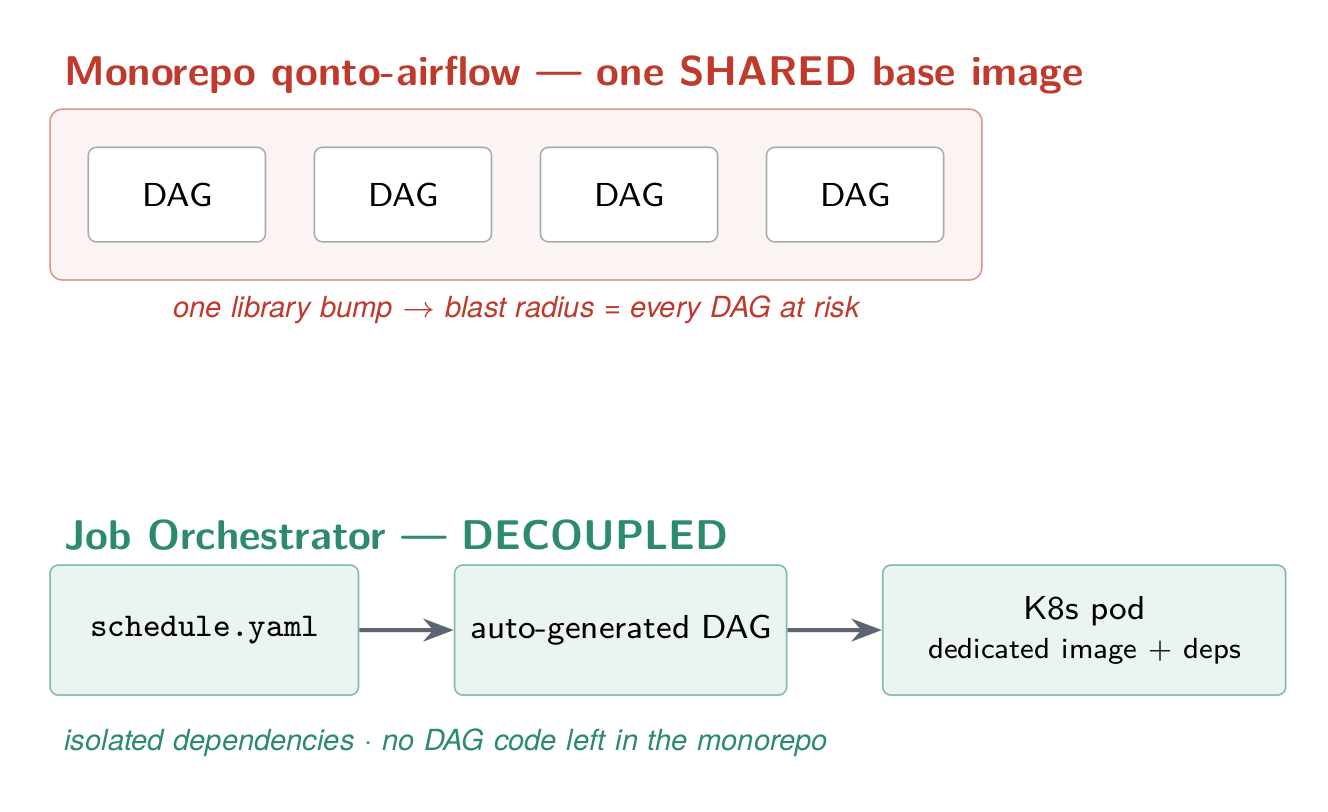
\includegraphics[width=0.8\textwidth]{imgs/job_orchestrator.png}
\caption{Airflow monorepo and the Job Orchestrator}
\label{fig:job-orch}
\end{figure}

\subsection{Data contracts: Qontract}\label{sec:qontract}

If config-driven generation is the \emph{mechanism}, \emph{Qontract} is the \emph{configuration} that sits behind every ingestion, and the reason the platform stays consistent from source to warehouse. A Qontract is a YAML \emph{data contract} (following the open ODCS~\texttt{v3.1.0} specification) that declares, for one table: its destination (Snowflake database and schema), its columns with both a \emph{logical} and a \emph{physical} type, its primary key, and an \texttt{ingestion} block telling the loader \emph{where} to read the source and \emph{how}. It is the single source of truth: the same file drives what is ingested, how each column is typed in Snowflake, and what the downstream dbt models and freshness tests expect. Listing~\ref{lst:qontract} shows a condensed real contract, the Notion \texttt{data\_bugs} board.

\begin{lstlisting}[language=yaml,caption={A contract example for the Notion data\_bugs table.},label={lst:qontract}]
apiVersion: 'v3.1.0'
kind: 'DataContract'
id: 'urn:datacontract:notion:raw:notion:data_bugs'
version: '1.0.0'
status: 'active'
servers:
  - { type: snowflake, database: raw, schema: notion }   # destination
schema:
  - name: 'data_bugs'
    logicalType: 'object'
    physicalType: 'table'
    properties:
      - { name: 'id',           logicalType: string,    physicalType: text,          primaryKey: true, required: true }
      - { name: 'Name',         logicalType: string,    physicalType: text }
      - { name: 'Status',       logicalType: string,    physicalType: text }
      - { name: 'created_time', logicalType: timestamp, physicalType: timestamp_ntz, required: true }
      - { name: 'Resolved At',  logicalType: date,      physicalType: date }
      - { name: 'archived',     logicalType: boolean,   physicalType: boolean,       required: true }
customProperties:
  - property: 'source_type'
    value: 'notion'
  - property: 'ingestion'
    value:
      page_size: 50
      resource_id: '2e7b3f6c73bc4dg49fef375e932d20e1'   # which Notion data source to read
\end{lstlisting}

Two things make the contract operational. First, the \texttt{ingestion} block is what the config-driven generator turns into a running job: \texttt{resource\_id} identifies the exact Notion data source to query and \texttt{page\_size} caps each API page. Second, the loader maps every property's declared type to a Snowflake type (Table~\ref{tab:type-map}); applying that mapping \emph{from the contract} rather than guessing it from the data is what guarantees a stable schema at every load. Chapter~\ref{ch:notion} shows the code that performs this parsing (\texttt{build\_resource\_from\_contract} and \texttt{yaml\_to\_dlt\_columns}).

\begin{table}[H]
\centering\small
\begin{tabular}{@{}lll@{}}
\toprule
\textbf{Contract} (logical / physical) & \textbf{Snowflake type} & \textbf{Example column} \\
\midrule
string / text & \texttt{TEXT} & \texttt{Name}, \texttt{Status} \\
timestamp / timestamp\_ntz & \texttt{TIMESTAMP\_NTZ} & \texttt{created\_time} \\
date / date & \texttt{DATE} & \texttt{Resolved At} \\
boolean / boolean & \texttt{BOOLEAN} & \texttt{archived} \\
number / number & \texttt{NUMBER(38,6)} & --- \\
array, object / variant & \texttt{VARIANT} & labels, people\dots \\
\bottomrule
\end{tabular}
\caption{How a Qontract property type maps to a Snowflake column type.}
\label{tab:type-map}
\end{table}

\section{My position and assignments}

Integrated into the team as a data engineer intern, I took ownership of topics end to end, from analysis to production. My three main assignments, presented in the following chapters, were: (i)~migrating Notion ingestion to the dlt framework; (ii)~migrating the Tableau pipelines out of the Airflow image with a move to JWT authentication; and (iii)~building the CESOP regulatory transmission chain for the Netherlands.
\chapter{State of the art and problem statement}\label{ch:sota}

The projects of this internship belong to data engineering and to software engineering applied to pipelines. This chapter situates the work with respect to the state of the art of integration paradigms, ingestion frameworks, orchestration, machine-to-machine authentication and warehouse loading. It concludes by formalising the problem common to the projects.

\section{Integration paradigms: from ETL to EL}

Data integration long followed the \emph{ETL} paradigm (\emph{Extract–Transform–Load}): data is extracted and transformed \emph{before} being loaded into a target database. The advent of elastic cloud warehouses such as Snowflake or BigQuery favoured the \emph{EL} (or \emph{ELT}) paradigm: the raw data is \emph{loaded first}, then transformed \emph{inside} the warehouse using tools such as dbt~\cite{dbt-docs}. Deferring transformation downstream offers several recognised advantages~\cite{kleppmann}: the raw data remains available (replayability), the transformation logic is versioned and tested like code, and extraction reduces to a faithful copy operation. Qonto's platform follows this paradigm: ingestion must produce a faithful mirror of the source in \texttt{RAW}, and all business logic lives in dbt. This separation has a direct consequence for the Notion project: an ingestion \emph{must not} alter the shape of the data, on pain of breaking the downstream dbt models.

\section{Ingestion frameworks: from the in-house operator to the declarative framework}

Three families of approaches coexist for extracting a source and loading it into a warehouse.

\paragraph{In-house operators.} Historically, Qonto wrote one Airflow \emph{operator} per source type (for example a \texttt{NotionToS3Operator}). This approach gives full control but places on the team the entire cross-cutting logic: pagination, error retries, typing, incremental loading, code that must be maintained and that is a recurring source of bugs.

\paragraph{Connector platforms.} Tools such as Airbyte~\cite{airbyte} provide a catalogue of ready-made connectors. They reduce the code to write but introduce heavy infrastructure (a service to operate) and impose their own destination formats and conventions, which complicates parity with an existing system.

\paragraph{``Library'' EL frameworks.} A more recent approach embeds ingestion as a \emph{library} inside a plain Python program. The \emph{dlt} (\emph{data load tool}) framework~\cite{dlt-docs} is a representative: the developer declares \emph{resources} (Python generators yielding records) and a \emph{pipeline} towards a \emph{destination} (Snowflake, say); the framework automatically handles API pagination, \emph{normalisation} of semi-structured data, file \emph{staging} and loading, including incremental loads and schema tracking. dlt thus offers the best of both worlds: little in-house code, yet without the infrastructure of a connector platform. At Qonto, dlt was already in production for other sources (LinkedIn and Facebook advertising), but with a \emph{data-lake} destination (Iceberg); using a native Snowflake destination was a first (Chapter~\ref{ch:notion}).

\section{Orchestration and infrastructure coupling}

Airflow~\cite{airflow-docs} models a pipeline as a directed acyclic graph (DAG) of tasks. A structuring design choice is how the \emph{code} and \emph{dependencies} of the tasks are packaged. A \emph{monorepo} with a Docker image shared by all DAGs simplifies deployment but creates strong coupling: any library upgrade potentially affects \emph{all} pipelines. This is the \emph{blast radius}: the more a dependency is shared, the wider the risk induced by changing it. Software engineering literature and practice recommend, to contain this risk (\emph{dependency isolation}) for example by running each job in its own container, via Airflow's \texttt{KubernetesPodOperator} or an equivalent pattern. Qonto's \emph{Job Orchestrator} (Chapter~\ref{ch:context}) applies exactly this principle. This coupling to the shared image is the common thread of the first two projects, formalised in \S\ref{sec:pb}.

\section{Machine-to-machine authentication}

Making two systems talk to each other without human intervention raises the question of authentication. Several mechanisms exist, of increasing stringency.

\paragraph{Personal access tokens (PAT).} A \emph{Personal Access Token} is a long-lived secret tied to an account. Simple to implement, it has two major flaws: its \emph{rotation} (renewal before expiry) is a recurring manual task and a source of incidents, and its nature as a durable secret increases the exposure surface. The Tableau project (Chapter~\ref{ch:tableau}) started from managing fourteen annually rotated PATs.

\paragraph{Short-lived signed tokens (JWT).} The \emph{JSON Web Token} standard~\cite{rfc7519} lets a client \emph{mint} its own signed token, with a very short lifetime, from a single secret. The \emph{JWT bearer} profile of OAuth~2.0~\cite{rfc7523} formalises exchanging that assertion for a session token. Tableau exposes this mechanism through its \emph{Connected Apps}~\cite{tableau-connectedapps}: a single secret, never transmitted over the network, replaces the multitude of PATs; each run mints a token valid for a few minutes, with least-privilege \emph{scopes}. This shift from a durable shared secret to a short-lived per-run token illustrates two best practices: \emph{least privilege} and \emph{reducing the lifetime of secrets}.

\paragraph{Mutual certificate authentication (mTLS/PKI).} In exchanges with public administrations, authentication often relies on a public-key infrastructure (PKI) and \emph{mutual TLS}: the client presents an X.509 certificate issued by a trusted authority. This is the model imposed by the Dutch Digipoort gateway via a PKIoverheid certificate, over an FTPS channel~\cite{rfc4217} and not to be confused with SFTP (Chapter~\ref{ch:cesop}).

A cross-cutting point across these mechanisms is \emph{secrets management}: no secret should be written in clear text in the code or the image. Qonto uses AWS SSM Parameter Store (encrypted), where only the parameter \emph{name} appears in the configuration, the value being resolved at runtime.

\section{Warehouse loading: staging, \texttt{COPY} and atomic swap}

Efficiently loading large volumes into Snowflake follows a well-established pattern~\cite{snowflake-copy}: drop the files on object storage (S3), then run a bulk \texttt{COPY INTO} command. The question of \emph{visibility} then arises while a table is being fully reloaded in ``replace'' mode. A naive approach (truncate then re-insert) leaves a window during which the table returns zero rows. The \emph{atomic swap} technique solves this: load into a \emph{staging} table, then exchange the two tables with an instantaneous metadata operation (\texttt{SWAP}), so that a reader sees the old version until commit, then the new one with no partial state. Two subtleties, central to Chapter~\ref{ch:notion}, accompany this pattern: Snowflake's \texttt{SWAP} operation \emph{also exchanges the grants} between the two tables.

\section{Regulatory reporting and data transmission}

Finally, part of the internship falls under \emph{compliance}. The European CESOP directive~\cite{cesop-eu} has, since 2024, required payment service providers to report their cross-border payments quarterly, in a standardised XML format, in order to fight VAT fraud. While most countries offer a web API, some, including the Netherlands, impose a government gateway (Digipoort) with a file-based exchange protocol and certificate authentication. Building such a chain is a problem of \emph{systems integration} and \emph{state machines} (submission, then asynchronous reconciliation of acknowledgements that may span several weeks) more than a data problem in the classical sense.

\section{Problem statement and positioning}\label{sec:pb}

From this state of the art, the internship's common problem emerges. In the first two projects, the business logic was not itself faulty; the true source of fragility was the \emph{coupling} to Airflow's shared Docker image, which made any change risky and concealed failures. The adopted approach is therefore, each time: (1)~\emph{diagnose} that the real constraint is infrastructural; (2)~\emph{decouple} the job into a dedicated repository and image (via the Job Orchestrator); (3)~take advantage of the decoupling to \emph{remove} a brittle legacy mechanism and \emph{harden} the job; all of it (4)~\emph{without interruption} for downstream consumers. The third project, regulatory in nature, applies the same demand for rigour and industrialisation to a brand-new chain. The following chapters unfold this approach project by project.

\chapter{Migrating Notion ingestion to dlt}\label{ch:notion}

This first project fully illustrates the approach outlined in \S\ref{sec:pb}: start from a production incident, trace it back to the infrastructure cause, decouple, then harden, all without interruption. It is also the project where the real difficulty turned out to be very different from the apparent one.

\section{The legacy}

Several business tables come from Notion databases (reference data, bug-tracking boards, control scopes, etc.). Their ingestion lived \emph{inside} \texttt{qonto-airflow}, as a chain of three in-house operators:

\begin{center}\small
\texttt{NotionToS3Operator} $\rightarrow$ \texttt{S3ToSnowflakeOperator} $\rightarrow$ \texttt{SwapSnowflakeTablesOperator}
\end{center}

The first operator (about 300 lines) extracted the whole Notion database and wrote a CSV to S3; the second loaded that CSV into a temporary table via \texttt{COPY INTO}; the third performed an atomic swap between the temporary table and the production table. Each table was described by a data contract (Qontract), a YAML declaring fields, types and primary key, which the operator read to know what to extract and how to type it. The \texttt{notion-client} library was installed \emph{in Airflow's shared base image}.

\section{The trigger: a silent-truncation incident}

In early 2026, the \texttt{notion-client} library was bumped from 0.9.0 to 3.0.0 in the base image. This bump introduced a breaking API change: the \texttt{databases.query} endpoint was replaced by \texttt{data\_sources.query} (Notion having split the notion of a ``database'' into one or more ``data sources''). But the old, now-deprecated endpoint \textbf{silently capped results at 300 rows} (six pages of fifty) by returning \texttt{has\_more=false} \emph{without raising an error}. The result: a \emph{silent data truncation} in production, undetected by the mechanisms in place.

Beyond the one-off bug, two \emph{structural} problems were identified during the value analysis:

\begin{enumerate}
  \item \textbf{Strong coupling} to the shared image: bumping \texttt{notion-client} is risky (blast radius = all DAGs) and slow.
  \item \textbf{No resilience} to silent failures: neither row-count validation nor alerting on truncation.
\end{enumerate}

The second point is the most instructive: the problem was not merely that a figure was wrong, but that the system was \emph{unable to detect it}. The right answer therefore could not be a simple one-off fix.

\section{Options considered and decision}

Three approaches, all based on decoupling from the base image, were compared (Table~\ref{tab:notion-options}).

\begin{table}[H]
\centering\small
\renewcommand{\arraystretch}{1.3}
\begin{tabularx}{\textwidth}{@{}p{3.1cm}Xc@{}}
\toprule
\textbf{Approach} & \textbf{Principle and trade-off} & \textbf{Chosen} \\
\midrule
Job Orchestrator (rewrite) & Code and dependencies in a dedicated repository. Requires \emph{rewriting by hand} the whole extract $\rightarrow$ S3 $\rightarrow$ \texttt{COPY} $\rightarrow$ swap chain. & No \\
Custom providers (\texttt{airflow-kube-pod-jobs}) & One image per job, but a \texttt{KubernetesPodOperator} \emph{still} has to be written and maintained in \texttt{qonto-airflow}: the orchestration-side coupling remains. & No \\
\textbf{dlt} (\texttt{qonto-python-dlt}) & EL framework already in production, same Job Orchestrator pattern, \emph{but} pagination, S3 staging, \texttt{COPY INTO}, atomic swap and load auditing provided \emph{natively}. & \textbf{Yes} \\
\bottomrule
\end{tabularx}
\caption{Comparison of the three decoupling approaches for Notion ingestion.}
\label{tab:notion-options}
\end{table}

The decisive argument: the rewrite approach would have had me re-code \emph{by hand} exactly what dlt already does; including pagination, which is precisely the fix for the truncation bug. dlt brought the \emph{same decoupling} with \emph{less in-house code} and \emph{free resilience}. The only net-new to take on was the, at Qonto unprecedented, use of dlt's Snowflake destination.

\begin{figure}[H]
\centering
\begin{tikzpicture}[
  font=\sffamily\scriptsize,
  box/.style={rectangle,rounded corners=2pt,draw=qgray!60,fill=qlight,minimum height=8mm,align=center,inner sep=3pt},
  old/.style={box,fill=white},
  new/.style={box,fill=qaccent2!14,draw=qaccent2!70,minimum height=9mm},
  arr/.style={-{Stealth[length=1.6mm]},draw=qgray,thick}
]
\node[old] (a) {NotionToS3\\Operator};
\node[old,right=6mm of a] (b) {S3To\\Snowflake};
\node[old,right=6mm of b] (c) {SwapSnowflake\\Tables};
\node[align=left,font=\sffamily\scriptsize\itshape,left=4mm of a] {Before\\(in the Airflow\\image):};
\draw[arr] (a)--(b); \draw[arr] (b)--(c);
\node[new,below=12mm of b] (d) {dlt \texttt{notion} job — one \texttt{pipeline.run()} call\\{\scriptsize extract (native pagination) $\rightarrow$ normalize $\rightarrow$ load (S3 staging + COPY + SWAP + audit)}};
\node[align=left,font=\sffamily\scriptsize\itshape,left=4mm of d.west,anchor=east] {After\\(dedicated repo):};
\draw[arr,draw=qaccent2] ($(a.south)!0.5!(c.south)$) -- (d.north);
\end{tikzpicture}
\caption{The Notion migration: Before \& after.}
\label{fig:notion-ba}
\end{figure}

\section{Implementation: the dlt architecture}

The job lives in \texttt{qonto-python-dlt/jobs/notion/}, split into tested modules (\texttt{main}, \texttt{contracts}, \texttt{helpers}, \texttt{formatters}, \texttt{naming}, \texttt{governance}). The entry point is \texttt{python -m jobs.notion.main --yaml <s3://\dots contract.yaml>}: \emph{one invocation = one contract = one table}. Figure~\ref{fig:notion-archi} gives the end-to-end picture across the six stages, from the contract down to post-load governance: \textbf{(1)}~the \emph{Qontract}, parsed into column hints, ingestion knobs and tag definitions; \textbf{(2)}~\emph{orchestration} as a per-table DAG (Job Orchestrator); \textbf{(3)}~\emph{extract \& normalize} via the dlt \texttt{notion\_pages} resource (REST client + cursor paginator, 19 property formatters, contract-driven type hints, \texttt{object/array} $\rightarrow$ VARIANT); \textbf{(4)}~\emph{durable staging} as JSONL on S3; \textbf{(5)}~\emph{warehouse load} (\texttt{COPY INTO} $\rightarrow$ atomic swap $\rightarrow$ \texttt{RAW.NOTION.<table>}, plus the dlt audit tables); \textbf{(6)}~\emph{post-load governance} (column tags applied from the contract).

\begin{figure}[H]
\centering
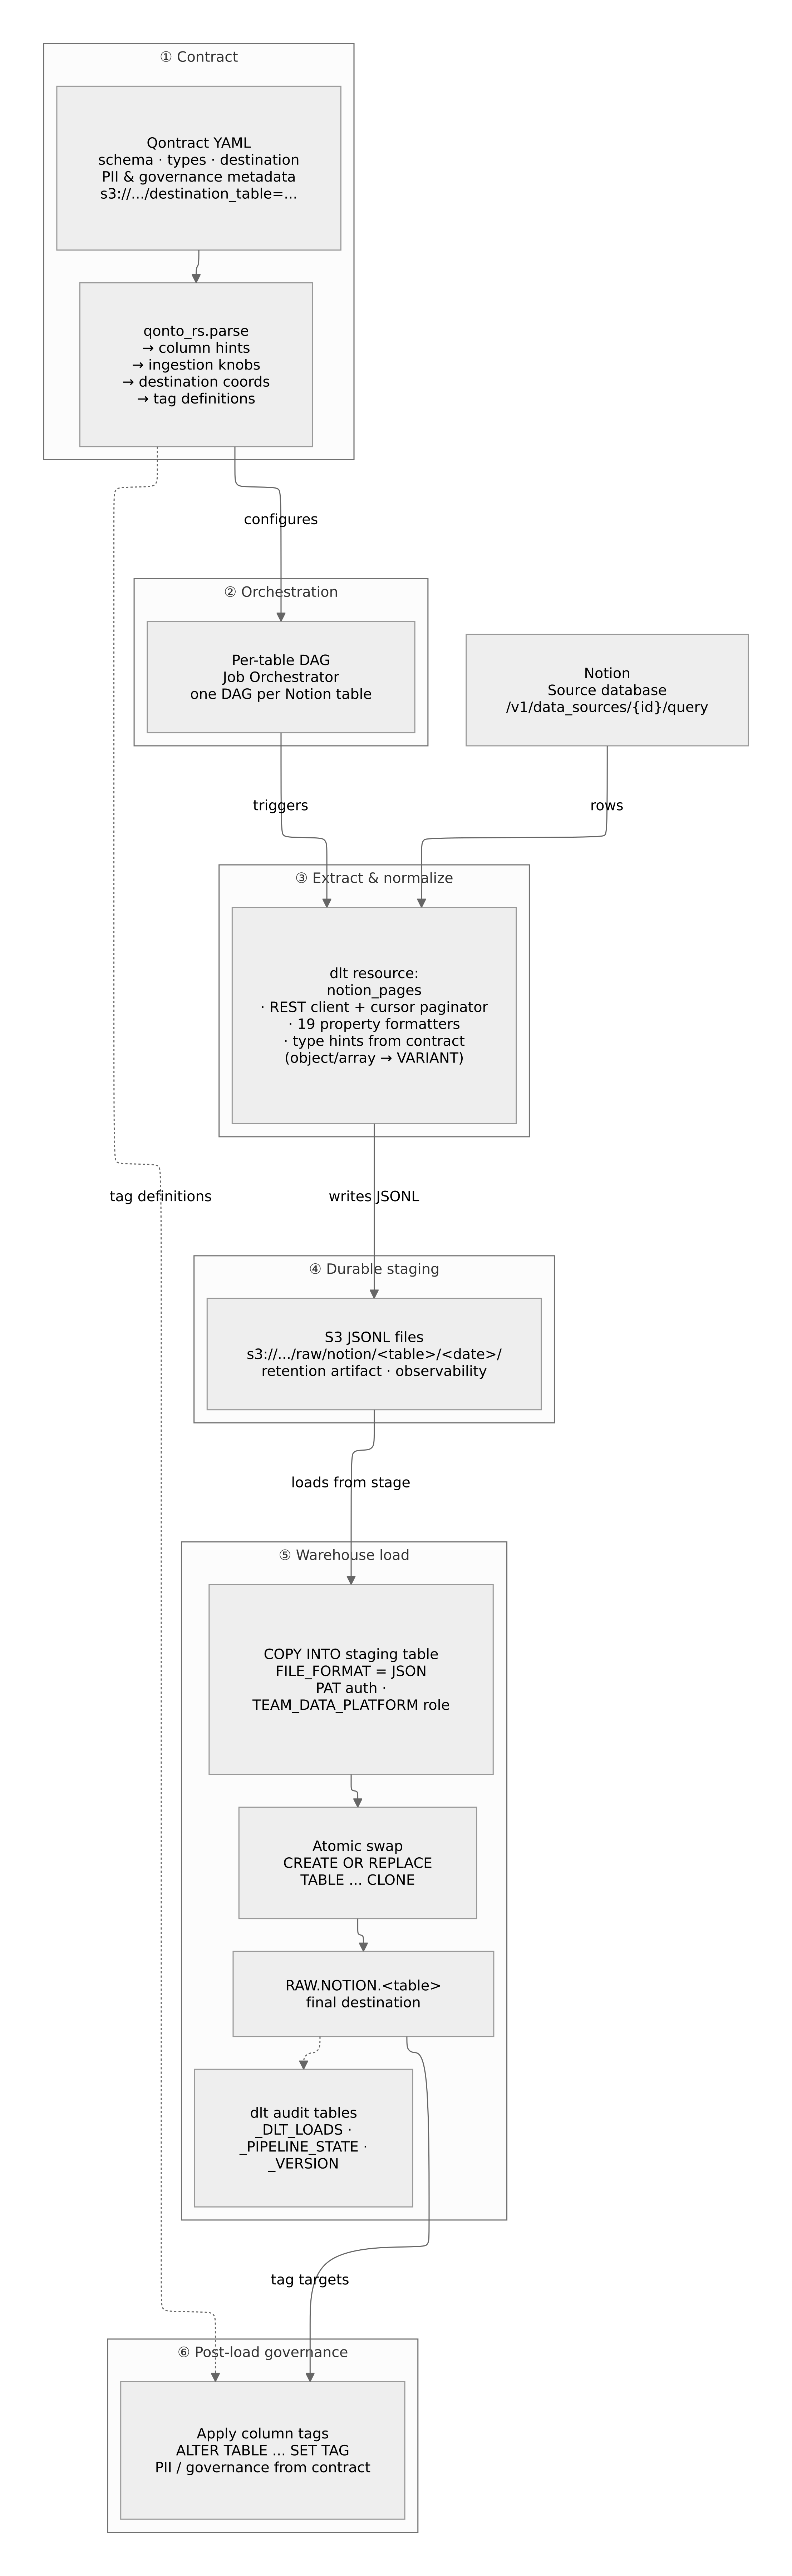
\includegraphics[height=0.95\textheight]{imgs/notion_archi.png}
\caption{End-to-end architecture of the Notion$\rightarrow$dlt pipeline.}
\label{fig:notion-archi}
\end{figure}

The pivotal function, \texttt{build\_resource\_from\_contract()}, is \emph{pure} (no I/O): it reads the YAML contract and derives from it the list of fields, the dlt \emph{column hints} via a \texttt{yaml\_to\_dlt\_columns()} translator, the table name and the primary key (the contract's, otherwise falling back to \texttt{id}), then builds the dlt resource, applying those hints with the ``replace'' write disposition. Listing~\ref{lst:notion-parse} shows this parsing: it is exactly the code behind the type mapping introduced in Chapter~\ref{ch:context} (Table~\ref{tab:type-map}).

\begin{lstlisting}[language=Python,caption={How a Qontract is parsed into a typed dlt resource.},label={lst:notion-parse}]
# contracts.py -- translate ONE contract field into a dlt column hint
def yaml_field_to_dlt_column(prop):
    # ODCS v3.1.0: resolve physicalType first (narrow, e.g. timestamp_ntz),
    # then fall back to logicalType (abstract, e.g. timestamp).
    if prop.physical_type in _LOGICAL_TYPE_TO_DLT:
        column = dict(_LOGICAL_TYPE_TO_DLT[prop.physical_type])
    else:
        column = dict(_LOGICAL_TYPE_TO_DLT[prop.logical_type])
    column["nullable"] = True            # legacy made every column nullable
    if prop.primary_key:
        column["primary_key"] = True
        column["nullable"] = False       # PK stays NOT NULL (Notion page id)
    return column

def yaml_to_dlt_columns(properties):
    # key by normalized (lowercased) name so dlt matches columns at load time
    return {normalize_column_name(p.name): yaml_field_to_dlt_column(p)
            for p in properties}

# main.py -- wire the parsed contract into a configured dlt resource (pure)
def build_resource_from_contract(contract, access_token, ...):
    schema      = contract.schema[0]
    source_id   = contract.get_custom("ingestion.resource_id")
    page_size   = contract.get_custom("ingestion.page_size")   # e.g. 50
    fields      = [p.name for p in schema.properties]
    columns     = yaml_to_dlt_columns(schema.properties)       # type hints
    primary_key = next((normalize_column_name(p.name)
                        for p in schema.properties if p.primary_key), "id")
    resource = notion_pages(source_id, access_token, fields, page_size)
    return resource.apply_hints(
        table_name=schema.name.lower(),
        columns=columns,               # types + nullability from the contract
        primary_key=primary_key,
        write_disposition="replace",   # full refresh -> atomic swap
    )
\end{lstlisting}

Two design choices in this parsing are worth noting. Resolving \texttt{physicalType} \emph{before} \texttt{logicalType} is what lets a \texttt{created\_time} field (\texttt{logicalType: timestamp}, \texttt{physicalType: timestamp\_ntz}) produce a \texttt{TIMESTAMP\_NTZ} column rather than a timezone-aware one; and forcing every column \texttt{nullable} (except the primary key) mirrors the legacy CSV$\rightarrow$VARCHAR pipeline, so a contract's \texttt{required:\ true} never aborts the load on the first NULL.

Everything then starts from \emph{a single call}, \texttt{pipeline.run()}, monolithic from the outside but internally chaining three phases:

\begin{enumerate}
  \item \textbf{Extract}: the resource queries \texttt{/v1/data\_sources/\{id\}/query} via dlt's REST client and its paginator. \emph{Pagination is delegated to the library}, which stops on the documented \texttt{has\_more=false}. \textbf{This is the underlying fix for the silent truncation}: an in-house paginator may terminate incorrectly and truncate silently. Records are buffered then written to local JSONL and nothing touches Snowflake yet.
  \item \textbf{Normalize}: dlt re-reads the JSONL, applies the contract's column hints, and rewrites the files. The format is forced to JSONL so that semi-structured columns land as \emph{native} VARIANT/ARRAY.
  \item \textbf{Load}: the only phase that talks to Snowflake. dlt generates the SQL sequence of Listing~\ref{lst:notion-sql}.
\end{enumerate}

\begin{lstlisting}[language=SQL,caption={SQL sequence generated by dlt during the load phase.},label={lst:notion-sql}]
-- 1) staging table typed by the contract's column hints
CREATE TABLE IF NOT EXISTS RAW.NOTION_STAGING.<TABLE> (...);
-- 2) bulk load from the JSONL on S3 (external stage)
COPY INTO RAW.NOTION_STAGING.<TABLE> FROM @<s3_stage>/... FILE_FORMAT=(TYPE=JSON);
-- 3) atomic swap (staging-optimized + enable_atomic_swap)
ALTER TABLE RAW.NOTION.<TABLE> SWAP WITH RAW.NOTION_STAGING.<TABLE>;
-- 4) load audit row
INSERT INTO RAW.NOTION._DLT_LOADS (load_id, schema_name, status, inserted_at) VALUES (...);
\end{lstlisting}

A methodological point I made sure to understand precisely: \emph{I write none of these queries}. dlt produces them from the destination configuration (atomic swap, ``staging-optimized'' strategy) and the column hints. My work consisted in \emph{choosing the right safe defaults} and \emph{constraining} the framework, not in rewriting the plumbing.

\section{The real challenge: byte-for-byte parity with the legacy}

The dlt pipeline was the easy part. The central technical difficulty was elsewhere: \textbf{producing output \emph{identical} to the legacy system's}, so that no downstream dbt model would break at cutover time. Left to its defaults, dlt would have drifted along several axes; I had to constrain it everywhere (Table~\ref{tab:parity}).

\begin{table}[H]
\centering\small
\renewcommand{\arraystretch}{1.3}
\begin{tabularx}{\textwidth}{@{}p{2.9cm}X@{}}
\toprule
\textbf{Axis} & \textbf{Constraint imposed for parity} \\
\midrule
Column naming & dlt normalises to \emph{snake\_case} (strips the trailing \texttt{\_}, collapses \texttt{\_\_}). I wrote a custom naming convention (\texttt{naming.py}, imposed before importing dlt) that reproduces exactly the legacy cleaning, transliterates accents/emojis and \emph{suffixes Snowflake reserved words with a} \texttt{\_} (\texttt{table}, \texttt{on}, \texttt{start}\dots). \\
Types & Contract $\rightarrow$ dlt-hints translator routing first by the \emph{physical type} (ODCS). \\
Values & Coercion by Notion property type: dates reduced to the local day, timestamps as local wall-clock time (offset stripped), integers rounded, decimals as \texttt{NUMBER(38,6)}, semi-structured kept native. \\
Nullability & All columns forced to \emph{nullable} (except the primary key), because the legacy load made everything nullable. \\
S3 layout & Same date partitioning as the legacy, preserving load history. \\
\bottomrule
\end{tabularx}
\caption{The five parity axes constrained to make the cutover invisible downstream.}
\label{tab:parity}
\end{table}

This is the project's key lesson: the real difficulty was not ``using dlt'', but \emph{guaranteeing zero drift} of schema or value relative to production, so that the cutover would be transparent to the hundreds of downstream dbt models. Each constraint in Table~\ref{tab:parity} corresponds to a real parity bug, diagnosed and then fixed, often at the cost of a fine investigation of both systems' behaviour.

\section{Two mechanisms re-implemented around dlt}

dlt provides pagination, staging and the swap ``for free'', but it does not reproduce two behaviours of the legacy swap that had to be preserved. I coded them around \texttt{pipeline.run()}.

\paragraph{(a) Grant preservation on the swap.} Snowflake's \texttt{SWAP WITH} operation \emph{also exchanges grants}: after the swap, consumer roles (dbt, BI tools) would lose access on every run. I reproduced the legacy operator's behaviour: read the grants (\texttt{SHOW GRANTS}) \emph{before} the load, then \emph{re-apply} them one by one \emph{after} the swap.

\paragraph{(b) Schema reconciliation on contract drift.} The ``replace'' disposition replaces \emph{rows}, not the \emph{schema}: dlt never re-types an existing column. If a contract re-types a field (for example \texttt{text} $\rightarrow$ \texttt{array}), dlt would keep the old type indefinitely. I wrote a drift detector (\texttt{DESC TABLE} compared to the contract's expected types) which, on a re-typing or a removed column, switches the run to a rebuild mode; otherwise the interruption-free atomic swap is preserved. The mechanism is \emph{fail-safe by default} (any introspection error $\rightarrow$ no destructive rebuild) and \emph{self-resolving}.

\section{The zero-downtime production cutover}

The trickiest part was not writing the pipeline, but \emph{cutting over production} without breaking the dbt consumers or the Airflow sensor logic. I achieved it through a \emph{sequence of backward-compatible PRs} in \texttt{qonto-airflow} (Figure~\ref{fig:cutover}).

\begin{figure}[H]
\centering
\begin{tikzpicture}[font=\sffamily\scriptsize,node distance=3mm,
  pstep/.style={rectangle,rounded corners=2pt,draw=qaccent!60,fill=qaccent!8,align=center,inner sep=4pt,text width=2.5cm,minimum height=12mm},
  arr/.style={-{Stealth[length=1.6mm]},draw=qgray,thick}]
\node[pstep] (s1) {\textbf{\#1419}\\wire the dlt loader \emph{alongside} the old one};
\node[pstep,right=of s1] (s2) {\textbf{\#1513}\\cutover: dlt takes over \texttt{RAW.NOTION} (+ transitional shims)};
\node[pstep,right=of s2] (s3) {\textbf{\#1511}\\repoint the sensors to the \texttt{load} task};
\node[pstep,right=of s3] (s4) {\textbf{\#1529}\\remove the transitional shims};
\node[pstep,right=of s4] (s5) {\textbf{\#1536}\\decommission the operator and dependency};
\draw[arr] (s1)--(s2); \draw[arr] (s2)--(s3); \draw[arr] (s3)--(s4); \draw[arr] (s4)--(s5);
\end{tikzpicture}
\caption{Zero-downtime cutover sequence, from wiring in parallel to decommissioning.}
\label{fig:cutover}
\end{figure}

The detail that makes the difference: the sensors always targeted \texttt{raw.notion.<table>}, with table name and cadence \emph{unchanged} so downstream saw nothing happen. That is the very definition of a zero-downtime migration. The final step removed the legacy operator (about 300 lines) and its tests (about 550 lines), an orphaned Airflow \emph{pool}, an obsolete environment \emph{mapping}, and above all the \texttt{notion-client} dependency from the base image.

\begin{keybox}[Results and evaluation]
\begin{itemize}
  \item \textbf{Silent truncation eliminated by construction}: pagination delegated to the library and a \texttt{\_dlt\_loads} audit table on every load.
  \item \textbf{Coupling removed}: no more \texttt{notion-client} dependency in the Airflow base image.
  \item \textbf{Cutover with no downtime and no dbt regression}: byte-for-byte parity verified (names, types, nullability, time zones, S3 layout).
  \item \textbf{Reduced debt}: removal of the three-operator chain, the orphaned pool and the associated tests (on the order of 850 lines removed on the \texttt{qonto-airflow} side).
  \item \textbf{Added robustness}: grants preserved on the swap, schema drift auto-reconciled, a dedicated per-module test suite.
\end{itemize}
\end{keybox}

\begin{contribbox}
I carried this project end to end: incident analysis, comparison of approaches, full development of the dlt job and its modules, resolution of the five parity axes, re-implementation of grants and schema reconciliation, and steering of the cutover PR sequence into production (\#1419 to \#1536). I also spotted two latent bugs in the legacy code while reading it (a loop variable used outside its loop, and an error on an empty Notion database). Ownership of the system was then transferred to the Data Engineering team.
\end{contribbox}

\chapter{Migrating the Tableau DAGs and JWT authentication}\label{ch:tableau}

The second project applies the same decoupling approach as the first, but with a different root cause: here, the central problem is \emph{authentication}. It shows how a seemingly minor constraint (tokens to renew) in fact forces a redesign of the execution architecture.

\section{The legacy}

Two families of Tableau pipelines lived in \texttt{qonto-airflow}:

\begin{itemize}
  \item \textbf{Refresh}: a DAG \texttt{daily\_refresh\_tableau\_workbooks} (03:00 UTC) recomputed \textbf{62 workbooks} every night, one task per workbook, each gated by sensors on the dbt models that feed it (about 140 deduplicated sensors). The priority (\emph{P1}) workbooks are critical and page the on-call rotation on failure.
  \item \textbf{Metadata loading}: four DAGs queried Tableau's \emph{Metadata} GraphQL API (workbooks, tables, views, revisions) into Snowflake via the extract $\rightarrow$ S3 $\rightarrow$ Snowflake chain.
\end{itemize}

\section{The central problem: authentication}

The whole thing relied on \textbf{fourteen personal access tokens} (PATs): ten for refresh and four for metadata \emph{expiring every year} and tracked \emph{by hand} in a Notion table. A missed rotation broke the nightly refresh. To stay under the \emph{concurrent-session limit per token} imposed by Tableau, the refresh used a \emph{pool of ten tokens} managed by an XCom mechanism detailed below. Finally, the version of the Tableau client (\emph{Tableau Server Client}, TSC) embedded in the Airflow image was \emph{too old} to support \emph{Connected Apps}: the move to JWT was therefore \emph{blocked} as long as the dependency stayed in the shared image. We find here, exactly, the coupling identified in Chapter~\ref{ch:sota}.

\subsection{The legacy XCom mechanism}

This mechanism deserves an explanation, as it illustrates a subtle piece of technical debt. XCom is the communication channel between Airflow tasks, designed to be \emph{immutable} (append-only). The legacy code diverted it to implement a token pool:

\begin{enumerate}
  \item an operator pushed, at the start of the DAG, the list of the ten available connection names (the ``whiteboard'' of free tokens);
  \item one sensor per workbook, running in a \emph{single-slot Airflow pool} (a \emph{mutex}), read the list, \emph{removed} a token and \emph{rewrote} the shortened list;
  \item the refresh operator used the acquired token;
  \item a release operator returned the token at the end of the run (even on failure).
\end{enumerate}

\emph{Why a single-slot mutex?} Because the 62 acquisitions run in parallel and all perform a \emph{read–modify–write} cycle on the same list: without serialisation, two tasks would take the same token (a \emph{race condition}). The mutex guarantees a single mutation at a time, to be distinguished from the \emph{parallelism of ten} (the number of tokens). Above all, to mutate an XCom value mid-run, the legacy code \emph{wrote directly to the} \texttt{xcom} \emph{table} of Airflow's metadata database which is a mutable state hacked into the heart of the scheduler, brittle and invisible to Airflow. This is the \emph{hack} that the migration removed.

\section{Solution: dedicated pods and a JWT Connected App}

The solution combines decoupling and an authentication redesign:

\begin{itemize}
  \item \textbf{Migration of both pipelines} to \texttt{qonto-python-data-engineering} (\texttt{jobs/tableau/}), run as \texttt{CustomJobKubernetesPodOperator} — one pod per workbook, thus \emph{outside} the Airflow image. The \texttt{apache-airflow-providers-tableau} provider is removed from \texttt{qonto-airflow}.
  \item \textbf{Replacement of the 14 PATs by a single JWT \emph{Connected App}.} A \texttt{make\_jwt()} function mints, on each run, an HS256 token (\texttt{exp} at 5 minutes, a unique anti-replay identifier, least-privilege scopes), signed by a single secret resolved from AWS SSM. The application identifiers are public; only the secret value is confidential and is never transmitted or committed. \textbf{One secret replaces fourteen PATs.}
  \item \textbf{Full removal} of the XCom pool, the mutex and the associated operators. The refresh DAG goes from \emph{five tasks per workbook to two} (dbt sensor $\rightarrow$ pod); metadata from \emph{three tasks to one pod} (Figure~\ref{fig:tableau-ba}).
  \item The configuration of the 62 workbooks is \emph{driven by Python modules} and the refresh \texttt{schedule.yaml} is \emph{generated}, with a continuous-integration test keeping generation and modules in sync.
\end{itemize}

\begin{figure}[H]
\centering
\begin{tikzpicture}[font=\sffamily\scriptsize,node distance=5mm,
  t/.style={rectangle,rounded corners=2pt,draw=qgray!60,fill=white,align=center,inner sep=3pt,minimum height=7mm},
  n/.style={t,fill=qaccent2!14,draw=qaccent2!70},
  arr/.style={-{Stealth[length=1.6mm]},draw=qgray,thick}]
\node[align=left,font=\sffamily\scriptsize\itshape] (lb) {Before\\(5 tasks):};
\node[t,right=6mm of lb] (i) {initialize\\tokens};
\node[t,right=of i] (ds) {dbt\\sensor};
\node[t,right=of ds] (aq) {acquire\\token};
\node[t,right=of aq] (rw) {refresh\\workbook};
\node[t,right=of rw] (rl) {release\\token};
\draw[arr] (i)--(ds); \draw[arr] (ds)--(aq); \draw[arr] (aq)--(rw); \draw[arr] (rw)--(rl);
\node[align=left,font=\sffamily\scriptsize\itshape,below=10mm of lb.west,anchor=west] (la) {After\\(2 tasks):};
\node[n,right=6mm of la] (ds2) {dbt sensor};
\node[n,right=of ds2] (pod) {refresh\_workbook (K8s pod, internal JWT)};
\draw[arr,draw=qaccent2] (ds2)--(pod);
\end{tikzpicture}
\caption{Refreshing a workbook: before and after.}
\label{fig:tableau-ba}
\end{figure}

\section{How the JWT works}

On each run, \texttt{make\_jwt} encodes an HS256 token carrying the issuer (client identifier), the audience (\texttt{tableau}), the subject (service account), the requested scopes, a unique identifier and a five-minute expiry; the header references the secret identifier (Listing~\ref{lst:make-jwt}). This token is passed to the Tableau client, whose authentication call returns a \emph{session token} (valid for up to 240 minutes of inactivity) used thereafter. The refresh requests only \texttt{tableau:tasks:run} and \texttt{tableau:content:read} (least privilege).

\begin{lstlisting}[language=Python,caption={Minting the short-lived Tableau JWT (\texttt{jobs/tableau/authentication.py}).},label={lst:make-jwt}]
def make_jwt(client_id, secret_id, secret_value, scopes):
    return jwt.encode(
        {
            "iss": client_id,                                  # Connected App client id
            "exp": datetime.now(UTC) + timedelta(minutes=5),   # short-lived
            "jti": str(uuid.uuid4()),                          # anti-replay id
            "aud": "tableau",
            "sub": TABLEAU_USER,                               # service account
            "scp": scopes,                                     # least privilege
        },
        secret_value,                                          # the ONE secret (AWS SSM)
        algorithm="HS256",
        headers={"kid": secret_id, "iss": client_id},
    )
\end{lstlisting}

\section{Difficulties encountered}

Three concrete obstacles had to be overcome, each instructive.

\paragraph{The jobs API blocked under JWT.} Tracking a refresh's progress used the \texttt{jobs} API, which returns a 401 error for a session issued by a Connected App. \emph{Fix}: detect the end of the refresh by \emph{polling} the workbook's last-update timestamp (\texttt{updated\_at}) every 30 seconds until it changes.

\paragraph{Refresh-pod starvation.} An initial global cap made the slots \emph{shared} between the 140 dbt sensors and the pods: a ready pod could wait up to 90 minutes. \emph{Fix}: a \emph{dedicated Airflow pool} (ten slots) bounding \emph{only} the refresh pods.

\paragraph{Idempotency on 409 and 429.} If a refresh is already queued (code 409, for example triggered manually from the UI), we do not re-trigger it: we wait for the one in flight. Rate limiting (code 429) was handled with a back-off; it is now avoided upstream by the pool of ten.

\begin{keybox}[Important nuance: the real constraint is server-side]
Tableau Cloud caps concurrent extract refreshes at \emph{ten} per site. After migration, I \emph{keep} this limit of ten, but via a \emph{simple Airflow pool} rather than through token scarcity. What disappears: token scarcity, the XCom mutex and manual rotation. In other words, the migration does not remove the server limit, it removes the \emph{brittle plumbing} that simulated it.
\end{keybox}

\section{Decisions and trade-offs}

\emph{Why not simply bump the TSC in the Airflow image?} Because the image is \emph{shared by all DAGs}: bumping the Tableau client risked breaking other providers and coupled a product library to the lifecycle of everyone's image. Moving the dependency into a dedicated repository and pods unblocks the JWT \emph{and} reduces the risk surface to the Tableau perimeter alone.

\emph{Accepted trade-offs:} one more repository, image and deployment pipeline, plus a \emph{cross-repo contract}. The gain; JWT unblocked, zero rotation, removal of the XCom hack far outweighs it.

\begin{keybox}[Results and evaluation]
\begin{itemize}
  \item \textbf{One secret instead of fourteen PATs}, and \emph{zero manual rotation}: the ``missed rotation $\rightarrow$ broken refresh'' incident class disappears.
  \item \textbf{Simplification}: refresh from 5 to 2 tasks per workbook, metadata from 3 tasks to 1 pod; removal of the token pool, the mutex and the XCom mutation hack.
  \item \textbf{Decoupling}: Tableau provider removed from the base image; execution in isolated pods.
  \item \textbf{Reduced debt}: on the order of 880 lines of legacy code removed.
  \item \textbf{Cleanly bounded concurrency}: still capped at ten (Tableau Cloud limit), but through an explicit pool.
\end{itemize}
\end{keybox}

\begin{contribbox}
I led the entire migration: design and implementation of the JWT authentication and its tests, porting of the refresh and metadata pipelines to pods, configuration-driven generation of the 62 workbooks, resolution of the three difficulties above, and decommissioning of the legacy runtime on the \texttt{qonto-airflow} side (PR~\#1633/\#1634). In addition, I tooled the onboarding of a new workbook via a \emph{skill} that validates, generates the configuration and opens the PR; a contribution to the team's automation culture.
\end{contribbox}

\chapter{CESOP Netherlands regulatory transmission chain}\label{ch:cesop}

The third project differs from the first two: it is not about migrating an existing system, but about \emph{building a brand-new} regulatory transmission chain. It draws more on systems and protocol engineering than on data engineering.

\section{Regulatory context}

Since 1~January 2024, the European \emph{CESOP} directive~\cite{cesop-eu} has required every payment service provider (PSP) to report its cross-border payments \emph{quarterly}, in order to fight VAT fraud in cross-border e-commerce. The regulatory trigger: as soon as a PSP executes more than 25 cross-border payments to the same payee in a quarter, all those payments must be reported; authorities then cross-check the data between member states. As Qonto is a PSP, this reporting is an already-running process for the countries where it operates. The new element: the opening of a Dutch IBAN, operational since December~2025, which makes the Netherlands a new reporting country, with a first affected quarter (Q4~2025). And \emph{the Netherlands does it differently from every other country} which is precisely the subject of this project.

\section{The Dutch specificity}

Where other countries accept submission via a web API (HTTPS + API key or OAuth), the Netherlands imposes a government gateway, \textbf{Digipoort} (operated by the agency Logius), with an entirely different technical stack (Table~\ref{tab:nl-delta}).

\begin{table}[H]
\centering\small
\renewcommand{\arraystretch}{1.3}
\begin{tabularx}{\textwidth}{@{}p{3.2cm}XX@{}}
\toprule
\textbf{Element} & \textbf{Other countries (ES/IT/FR/DE)} & \textbf{Netherlands} \\
\midrule
Submission point & National tax portal & The \textbf{Digipoort} gateway \\
Authentication & API key / OAuth & \textbf{PKIoverheid} certificate (X.509), \textbf{mTLS} \\
Transmission & HTTPS POST & \textbf{FTPS} + a \texttt{.meta} companion file \\
Feedback & Direct API response & \textbf{Files dropped} into an \texttt{out/} folder to be polled (hours to weeks) \\
\bottomrule
\end{tabularx}
\caption{The gap between the usual CESOP submission and the Dutch route (Digipoort).}
\label{tab:nl-delta}
\end{table}

The most important design point is the distinction between \emph{the what} and \emph{the how}. \emph{The what} — the XML content (payments, payees, amounts) — is the \emph{payload}, produced by an existing generator in the Data Engineering team; it \emph{arrives as an input} to my project and follows the standard CESOP format (version~4.03). \emph{The how} — authenticate, attach a \texttt{.meta}, transmit, reconcile the acknowledgements — is my scope: the ``plumbing'' (\emph{transport/plumbing}). I build the pipes, not the water flowing through them.

\section{Architecture: two DAGs and a state table}

The ``submission $\rightarrow$ acknowledgement'' loop is \emph{asynchronous} and may span hours to weeks: a single task therefore cannot stay blocked waiting. The design splits the work into two DAGs, linked by a Snowflake state table (Figure~\ref{fig:cesop-dags}).

\begin{figure}[H]
\centering
\begin{tikzpicture}[font=\sffamily\scriptsize,node distance=2.6mm,
  st/.style={rectangle,rounded corners=2pt,draw=qaccent!60,fill=qaccent!8,align=left,inner sep=3pt,text width=4.6cm,minimum height=6mm},
  su/.style={rectangle,rounded corners=2pt,draw=qaccent2!60,fill=qaccent2!10,align=left,inner sep=3pt,text width=4.6cm,minimum height=6mm},
  db/.style={cylinder,shape border rotate=90,aspect=0.25,draw=qgray!70,fill=qlight,align=center,inner sep=3pt,minimum width=2.4cm},
  arr/.style={-{Stealth[length=1.6mm]},draw=qgray,thick}]
\node[st] (a1) {\textbf{DAG A — \texttt{cesop\_nl\_submit}} (quarterly)};
\node[st,below=of a1] (a2) {1. fetch the payload(s)};
\node[st,below=of a2] (a3) {2. validate (XSD)};
\node[st,below=of a3] (a4) {3. compute digest + build the \texttt{.meta}};
\node[st,below=of a4] (a5) {4. upload over FTPS (payload then \texttt{.meta})};
\node[st,below=of a5] (a6) {5. record the submission};
\draw[arr] (a1)--(a2);\draw[arr](a2)--(a3);\draw[arr](a3)--(a4);\draw[arr](a4)--(a5);\draw[arr](a5)--(a6);
\node[su,right=22mm of a1] (b1) {\textbf{DAG B — \texttt{poll\_receipts}} (every 3h)};
\node[su,below=of b1] (b2) {1. list open submissions};
\node[su,below=of b2] (b3) {2. fetch receipts (\texttt{out/})};
\node[su,below=of b3] (b4) {3. parse and classify};
\node[su,below=of b4] (b5) {4. update state};
\node[su,below=of b5] (b6) {5. alert on error (Slack)};
\draw[arr] (b1)--(b2);\draw[arr](b2)--(b3);\draw[arr](b3)--(b4);\draw[arr](b4)--(b5);\draw[arr](b5)--(b6);
\node[db,below=8mm of $(a6)!0.5!(b6)$] (state) {\texttt{RAW.CESOP\_NL.}\\\texttt{SUBMISSIONS}};
\draw[arr] (a6) |- (state);
\draw[arr] (state) -| (b2);
\draw[arr,dashed,draw=qgray] (b5) |- (state);
\end{tikzpicture}
\caption{Two-DAG architecture: a quarterly submitter and a three-hourly receipt poller, linked by a state table.}
\label{fig:cesop-dags}
\end{figure}

The \texttt{RAW.CESOP\_NL.SUBMISSIONS} table holds one row per submission and tracks its lifecycle: transport status, technical validation (a few hours), then business validation (days to weeks). DAG~A inserts the rows; DAG~B updates them as acknowledgements arrive.

\section{Implementation}

The job lives in \texttt{qonto-python-data-engineering/jobs/cesop\_nl/}, following the repository's conventions (\texttt{config.py} with Pydantic settings, \texttt{main.py}, \texttt{queries/}) and organised by responsibility:

\begin{itemize}
  \item \texttt{transport/} — the \textbf{FTPS/mTLS} client to Digipoort (connect, upload the file pair, list and download acknowledgements) and the \textbf{\texttt{.meta} builder} compliant with the \texttt{metabestand.xsd} schema;
  \item \texttt{submit/} — DAG~A's flow (fetch, validate, digest, \texttt{.meta}, upload, record);
  \item \texttt{poll/} — DAG~B's flow, with an \textbf{acknowledgement parser} that classifies the four artefact types in the \texttt{out/} folder into a uniform result, and the archival of raw receipts on S3;
  \item \texttt{state/} — the Snowflake state-table repository and its schema.
\end{itemize}

A few notable implementation points. The \texttt{.meta} file is a small XML that accompanies each payload: it carries the reference identifier (equal to the exact payload filename), the sender, the fixed receiver for CESOP and the size. The upload order is \emph{strict}: the payload first, \emph{then} the \texttt{.meta}, in the same session — it is the arrival of the \texttt{.meta} that triggers processing on the Digipoort side. Trusting Logius's server certificate required explicitly installing the certificate-authority chain. Rejection alerts are surfaced on Slack in \emph{Block Kit} format. Finally, \emph{resubmission} handling was implemented: a rejected delivery must be resent as a \emph{fresh initial submission} (not as a correction), with a file-identifier increment and dated archival of the acknowledgements.

\section{Sticking points resolved}

The analysis phase resolved several uncertainties, by reading the official specifications (Logius FTPS interface, the tax authority's ``dialogue'' document, the PSPNL manual):

\begin{itemize}
  \item \textbf{``Signing'' = computing a digest, not signing the XML.} The certificate is used for TLS authentication; integrity is provided by an optional \emph{SHA-512} digest in the \texttt{.meta}. No XML signature (XMLDSig) is required — a major simplification confirmed with the regulatory side, which avoids a heavy cryptographic dependency.
  \item \textbf{The format is not a ``PSPNL wrapper''.} The payload is standard CESOP~4.03; the Dutch specificity lives only in the \texttt{.meta} and the transport.
  \item \textbf{Dedicated ports.} CESOP does not use port~21: control port~4022, passive data ports 4023--4073, TLS~1.2 — which requires an \emph{egress allow-list} covering those ports.
  \item \textbf{A quarter may produce several files} (a 100~MB split rule): the job handles a \emph{list} of payloads, not a single file.
  \item \textbf{Resubmission model} (\texttt{CESOP100} new / \texttt{CESOP101} correction / \texttt{CESOP102} nil return): the correlation keys (message and document identifiers) that DAG~B must persist and match were identified.
\end{itemize}

\begin{keybox}[State of progress at the end of the internship]
\textbf{Done:} overall design and blueprint; \texttt{.meta} builder; Digipoort FTPS client; acknowledgement parser; Snowflake state model; submission flow (DAG~A) and polling flow (DAG~B); Logius CA trust; DAG scheduling; Slack alerts; resubmission handling. Almost everything could be built and tested \emph{offline} against local examples (about 80\%).\\[3pt]
\textbf{Remaining:} locating the certificate's private key and provisioning the secrets in SSM; opening the egress allow-list (SRE); the test campaign — \emph{ASD} (connectivity) then \emph{VTS} (validation) — before go-live and the first real delivery.
\end{keybox}

\begin{contribbox}
I handled the analysis (reading and synthesising the official specifications, resolving the sticking points) then the design and implementation of the entire transport chain: package structure, \texttt{.meta} builder, FTPS/mTLS client, acknowledgement parser, state model, and both end-to-end flows, through to scheduling, S3 archival and Slack alerts. I collaborated with the \emph{Regulatory} team (specifications, certificate) and \emph{SRE} (networking) for the dependencies outside my scope.
\end{contribbox}

\chapter{Assessment and skills acquired}\label{ch:assessment}

This chapter steps back from the three projects to draw out the skills acquired and the common methodological pattern.

\section{A common pattern: diagnose, decouple, harden}

The three projects share the same outline, summarised in Table~\ref{tab:synthesis}. The first two are migrations: the true source of fragility was not the business logic but a shared infrastructure dependency, and the right answer was to \emph{decouple} before \emph{hardening}, without ever interrupting the service. The third, regulatory in nature, applies the same rigour to a brand-new chain.

\begin{table}[H]
\centering\small
\renewcommand{\arraystretch}{1.35}
\begin{tabularx}{\textwidth}{@{}p{2.6cm}XX@{}}
\toprule
\textbf{Axis} & \textbf{Notion project} & \textbf{Tableau project} \\
\midrule
Triggering constraint & \texttt{notion-client} 0.9$\rightarrow$3.0 in the base image: breaking API + silent truncation & Tableau client too old in the base image: JWT blocked \\
Legacy fragility & No truncation detection & 14 manually rotated PATs + token pool + XCom hack \\
% Decoupling & To \texttt{qonto-python-dlt} (dlt Snowflake destination) & To \texttt{qonto-python-data-engineering} (K8s pods) \\
Real difficulty & Byte-for-byte parity + zero-downtime cutover & Unblocking the JWT by moving the dependency out + avoiding pod starvation \\
Resilience gained & Native pagination, load auditing. & A single secret, no more rotation \\
\bottomrule
\end{tabularx}
\caption{Summary of the pattern common to the two migrations.}
\label{tab:synthesis}
\end{table}

\section{Technical skills}

This internship let me consolidate and acquire a set of production-grade data-engineering skills:

\begin{itemize}
  \item \textbf{Ingestion and warehousing}: command of the EL paradigm, of the dlt framework (resources, pipelines, column hints, write dispositions), and of Snowflake loading mechanisms (S3 staging, \texttt{COPY INTO}, atomic swap, grant handling).
  \item \textbf{Orchestration}: designing Airflow DAGs, decoupling patterns via Kubernetes pods, sensors and dependency management, concurrency pools.
  \item \textbf{Security and authentication}: implementing JWT authentication (Connected App), understanding the PAT, OAuth and mTLS/PKI models, and secrets management through an encrypted parameter store.
  \item \textbf{Software quality}: per-module unit tests, continuous integration, linting, configuration validation, and tooling to automate recurring tasks.
  \item \textbf{Systems integration}: transport protocols (FTPS/mTLS), XML formats and schema validation.
\end{itemize}

\section{Methodological skills}

Beyond the technical side, the internship reinforced a way of working: \emph{trace problems back to the root cause} before coding (both migrations were born from a refusal to treat a symptom); \emph{make trade-offs explicit} rather than suffer them (choice of dlt, the Tableau server limit); \emph{design for reversibility and zero interruption}; and \emph{measure} the effect of changes (tasks reduced, an incident class eliminated). The team's \emph{Value Analysis / Value Engineering} approach served as a guiding thread for each of these points.

\section{Transferable skills}

I gained autonomy and \emph{ownership}: taking a high-impact topic and carrying it into production entails real responsibility, especially for critical pipelines that page the on-call rotation. Collaboration was essential: demanding code reviews, exchanges with different teams by documenting decisions, sticking points and trade-offs on Notion, both to transfer ownership of the systems to the team.

\section{Value for the company}

The deliverables carry direct and lasting value: the removal of two incident classes (silent truncation; missed token rotation), a significant reduction of legacy code and of coupling to the shared image, and the establishment of a non-existent regulatory chain. Beyond that, the patterns established (dlt's first Snowflake destination, a zero-downtime migration template, reusable JWT authentication) are references for the team's future migrations.

\chapter*{Conclusion and perspectives}
\addcontentsline{toc}{chapter}{Conclusion and perspectives}
\markboth{Conclusion and perspectives}{}

This end-of-studies internship, carried out within Qonto's Data Platform team, aimed to harden and industrialise business-critical data pipelines. The problem posed in the introduction — how to harden pipelines with no service interruption when the real source of fragility is a shared infrastructure dependency — found a coherent answer across three projects.

The first two, migrating Notion ingestion to dlt and migrating the Tableau pipelines to JWT authentication, validated the same approach: diagnosing that the coupling to Airflow's shared Docker image was the true constraint, decoupling the job into a dedicated repository and image, then removing a brittle legacy mechanism — a chain of operators with no truncation detection in one case, a token pool and an XCom hack in the other. In both cases the decisive difficulty was not writing the new code, but \emph{achieving the cutover without downstream consumers noticing}: byte-for-byte parity with production for Notion, mastery of concurrency and of the new authentication for Tableau. The third project, the CESOP transmission chain to the Dutch Digipoort gateway, applied the same rigour to a systems-integration and compliance problem, and was being finalised at the end of the internship.

In terms of results, this work eliminated two incident classes by construction, removed all manual secret rotation, took a risky dependency out of the shared image, and appreciably reduced legacy code and the number of Airflow tasks, while giving the company a new regulatory capability.

Several \textbf{perspectives} naturally extend these projects. For Notion ingestion, adding \emph{freshness tests} and volume checks would complement the resilience already gained, and dlt's Snowflake destination — inaugurated here — could be generalised to other sources currently carried by in-house operators. For Tableau, the JWT authentication template and the workbook-onboarding tooling can be reused beyond the current perimeter. For CESOP, the next step is the test campaign (\emph{ASD} connectivity then \emph{VTS} validation), the go-live, and monitoring the first real delivery through the business-validation window that may span several weeks. Finally, the \emph{zero-downtime decoupling} pattern established during this internship is a template transferable to the platform's future migrations.

On a personal level, this internship was a full immersion in production-scale data engineering: it taught me to favour root-cause diagnosis over symptom fixing, to explicitly own engineering trade-offs, and to measure the value of my work — all reflexes I consider the main takeaway of this experience.

\begin{thebibliography}{99}
\addcontentsline{toc}{chapter}{Bibliography}
\markboth{Bibliography}{}
\small

\bibitem{kleppmann} M.~Kleppmann, \emph{Designing Data-Intensive Applications}, O'Reilly Media, 2017.

\bibitem{dlt-docs} dltHub, \emph{dlt --- data load tool: Documentation}, 2026. \url{https://dlthub.com/docs}

\bibitem{dbt-docs} dbt Labs, \emph{dbt Documentation}. \url{https://docs.getdbt.com}

\bibitem{airflow-docs} Apache Software Foundation, \emph{Apache Airflow Documentation}. \url{https://airflow.apache.org/docs/}

\bibitem{airbyte} Airbyte, \emph{Airbyte Documentation}. \url{https://docs.airbyte.com}

\bibitem{snowflake-copy} Snowflake Inc., \emph{COPY INTO <table> --- Snowflake Documentation}. \url{https://docs.snowflake.com/en/sql-reference/sql/copy-into-table}

\bibitem{tableau-connectedapps} Tableau (Salesforce), \emph{Configure Tableau Connected Apps with Direct Trust}. \url{https://help.tableau.com/current/online/en-us/connected_apps.htm}

\bibitem{rfc7519} M.~Jones, J.~Bradley, N.~Sakimura, \emph{JSON Web Token (JWT)}, RFC~7519, IETF, May~2015. \url{https://www.rfc-editor.org/rfc/rfc7519}

\bibitem{rfc7523} M.~Jones, B.~Campbell, C.~Mortimore, \emph{JSON Web Token (JWT) Profile for OAuth~2.0 Client Authentication and Authorization Grants}, RFC~7523, IETF, May~2015. \url{https://www.rfc-editor.org/rfc/rfc7523}

\bibitem{rfc4217} P.~Ford-Hutchinson, \emph{Securing FTP with TLS}, RFC~4217, IETF, October~2005. \url{https://www.rfc-editor.org/rfc/rfc4217}

\bibitem{cesop-eu} Council of the European Union, \emph{Council Directive (EU) 2020/284 amending Directive 2006/112/EC as regards introducing certain requirements for payment service providers (CESOP)}, 2020. \url{https://eur-lex.europa.eu/eli/dir/2020/284}

\bibitem{qonto-press} R.~Dillet, \emph{French B2B fintech Qonto reaches 600,000 customers and files for a banking license}, TechCrunch, July~2025. \url{https://techcrunch.com/2025/07/02/french-b2b-fintech-qonto-reaches-600000-customers-files-for-banking-license}

\bibitem{qonto-wiki} Wikipedia, \emph{Qonto}, accessed 2026. \url{https://en.wikipedia.org/wiki/Qonto}

\end{thebibliography}

\appendix
\chapter{Detailed presentation of Qonto}\label{anx:qonto}

Qonto is a European neobank for professionals (freelancers, very small businesses and SMEs), founded in 2017 by Alexandre Prot and Steve Anavi and operated by the company Olinda~SAS~\cite{qonto-wiki}. Its offering covers the business account, payment cards, transfers, invoicing and pre-accounting and financial-steering tools. At the time of the internship, the company reports on the order of 600{,}000 customers, operates in eight European countries (France, Germany, Italy, Spain, Austria, Belgium, the Netherlands, Portugal) and states the ambition of reaching two million customers by 2030~\cite{qonto-press}. On the regulatory side, Qonto operates as a payment institution and has begun the process of obtaining a banking licence. This payment-service-provider status underpins the regulatory-reporting obligations discussed in Chapter~\ref{ch:cesop}.

\chapter{Technical environment and repositories}

The projects span several repositories:

\begin{description}[style=nextline,leftmargin=1em,font=\ttfamily\bfseries]
  \item[qonto-airflow] Airflow monorepo (declarative DAG generation, shared Docker base image). Target of the decommissionings and production cutovers.
  \item[qonto-python-dlt] dlt-based ingestion repository (Snowflake destination). Home of the new Notion job.
  \item[qonto-python-data-engineering] \emph{Job Orchestrator}: Python jobs run in Kubernetes pods. Home of the Tableau and CESOP jobs.
  \item[data-contracts] Data contracts (Qontract, YAML) describing the schema of ingested tables.
\end{description}

\noindent\textbf{Technical stack:} Apache Airflow (orchestration), Snowflake (warehouse), Amazon S3 (staging), dbt (transformation), Kubernetes (isolated execution), AWS SSM Parameter Store (secrets), Python~3.12, \texttt{uv} (dependency management).

\chapter{Main contributions (Pull Requests)}

As concrete evidence of the work carried out, the main merged PRs, by project.

\paragraph{Notion project (\texttt{qonto-python-dlt}).} Porting of the tested modules (\#46) and wiring of the test DAGs (\#47); naming conventions for parity (\#55, \#56, \#57); JSONL loading for native VARIANT/ARRAY (\#68); date and time-zone parity (\#70, \#79); serialisation of list/object columns (\#71, \#72, \#73); nullability aligned with the legacy (\#75); tuned retry session for long fetches (\#80); reserved-keyword suffixing (\#82); schema reconciliation on contract drift (\#83, \#84).

\paragraph{Notion project --- cutover (\texttt{qonto-airflow}).} Wiring the dlt loader in parallel (\#1419); cutover to \texttt{RAW.NOTION} (\#1513); repointing the sensors (\#1511); removing the transitional shims (\#1529); decommissioning the legacy operator and removing the \texttt{notion-client} dependency (\#1536).

\paragraph{Tableau project (\texttt{qonto-python-data-engineering}).} JWT dependencies and logic (\#171, \#173); metadata loader (\#179, \#180); refresh pipeline with generated schedule (\#187); concurrency cap and 409 idempotency (\#191); workbook-onboarding skill (\#194); publishing the priority seed to S3 (\#196); documentation (\#204).

\paragraph{Tableau project --- cutover (\texttt{qonto-airflow}).} Per-task priority from \texttt{schedule.yaml} (\#1593); per-DAG \texttt{max\_active\_tasks} (\#1602); P2 priority seed from S3 (\#1626); removal of the legacy refresh runtime --- operator, tokens, PATs, pool (\#1633, \#1634).

\paragraph{CESOP project (\texttt{qonto-python-data-engineering}).} Project blueprint (\#221); \texttt{.meta} builder (\#222); acknowledgement parser (\#224); Snowflake state model (\#225); Digipoort FTPS client (\#226); submission flow --- DAG~A (\#228); Logius CA trust (\#229); polling flow --- DAG~B (\#230).

\chapter{Code excerpts}

\section*{JWT authentication (Tableau project)}
The function that mints the short-lived HS256 token for the Tableau \emph{Connected App} (Chapter~\ref{ch:tableau}):

\begin{lstlisting}[language=Python,caption={\texttt{make\_jwt}: minting a short JWT signed by a single secret.}]
def make_jwt(client_id: str, secret_id: str, secret_value: str, scopes: list[str]) -> str:
    return jwt.encode(
        {
            "iss": client_id,
            "exp": datetime.now(UTC) + timedelta(minutes=5),
            "jti": str(uuid.uuid4()),          # anti-replay
            "aud": "tableau",
            "sub": TABLEAU_USER,
            "scp": scopes,                       # least privilege
        },
        secret_value,
        algorithm="HS256",
        headers={"kid": secret_id, "iss": client_id},
    )
\end{lstlisting}

\section*{Naming convention for parity (Notion project)}
The custom naming convention imposed on dlt to preserve production column names (Chapter~\ref{ch:notion}): it merely lowercases, without touching underscores, and declares itself case-insensitive to emit unquoted DDL.

\begin{lstlisting}[language=Python,caption={``Passthrough'' naming convention (excerpt).}]
class NamingConvention(BaseNamingConvention):
    # dlt collapses "__" ; we pick an out-of-band separator to
    # avoid the collision with Notion column names.
    PATH_SEPARATOR: ClassVar[str] = "\u25b6"   # out-of-band separator (U+25B6)

    def normalize_identifier(self, identifier: str) -> str:
        identifier = super().normalize_identifier(identifier)
        return self.shorten_identifier(identifier.lower(), identifier, self.max_length)

    @property
    def is_case_sensitive(self) -> bool:
        return False
\end{lstlisting}

\end{document}
